\chapter{在线编程评测平台系统验证}

\section{测试环境与验证维度}

系统测试的主要目的是回答一个比较实际的问题：本文实现的系统是否已经能够稳定跑通在线评测平台的核心流程。由于本文面向程序设计教学场景，因此测试重点不放在大规模性能压测上，而是放在题目读取、代码提交、判题状态返回、结果追踪以及 AI 辅助反馈是否基本可用这些关键环节上。

本次进行的测试对操作系统、Node.js 版本、数据库版本、Docker 运行环境、异步任务与实时推送组件、测试所使用的浏览器、AI 服务接入方式等关键信息都予以记录，目的在于确保论文里关于测试环境的描述能够和实际演示环境达成一致。

\begingroup
\small
\setlength{\LTleft}{\fill}
\setlength{\LTright}{\fill}
\setlength{\tabcolsep}{2pt}
\begin{xltabular}{\textwidth}{P{0.20\textwidth}>{\RaggedRight\arraybackslash}X}
\caption{测试环境配置}\\
\toprule
项目 & 配置 \\
\midrule
\endfirsthead
\multicolumn{2}{c}{续表\thetable}\\
\toprule
项目 & 配置 \\
\midrule
\endhead
\bottomrule
\endfoot
操作系统 & macOS 26.2 \\
Node.js 版本 & v25.8.1 \\
Bun 版本 & 1.3.1 \\
Next.js 版本 & 15.1.7 \\
数据库 & PostgreSQL \\
ORM / Prisma 版本 & Prisma 6.7.0 \\
异步任务组件 & Inngest，本地服务通过 \path{/api/inngest} 注册事件函数 \\
实时推送组件 & Soketi / Pusher-compatible WebSocket 服务 \\
缓存与任务基础设施 & Redis 7 \\
容器环境 & Docker 28.3.3 \\
支持语言 & C、C++ \\
AI 服务 & DeepSeek，通过 @ai-sdk/openai-compatible 接入 \\
浏览器 & Google Chrome \\
\bottomrule
\end{xltabular}
\endgroup

表里这些环境参数都来自本次项目的实际测试环境，覆盖了本机运行时版本和关键依赖配置。把这些信息明确写出来，主要是为了让论文描述和演示环境能够一一对应，也方便他人在复核时做差异排查。

本章中的截图、状态返回结果和 AI 分析案例，主要围绕核心流程、判题状态、AI 反馈、界面交互和工程构建结果展开。

\section{核心功能验证}

功能测试主要围绕用户登录、题目浏览、题目详情展示、模板加载、代码提交、提交记录查看、判题结果展示和 AI 辅助反馈等核心功能展开，并采用黑盒测试思路，对输入操作、系统响应和最终页面结果进行逐项核验。对于题库管理相关页面，测试同时覆盖题目内容读取、测试数据关联以及不同语言模板加载情况。

本文按测试项、输入或操作、预期结果与实际结果四列的形式整理功能测试表，以便将测试步骤、页面证据与最终结论进行一一对应。

功能测试并不追求把所有页面都列一遍，而是优先覆盖系统核心流程上的关键节点。对本文系统来说，更重要的是证明系统能否顺利完成一次完整的做题和判题过程，即从登录进入系统，到加载题目、提交代码、查看结果，再到读取 AI 分析，这条链路是否真正跑通。

\begingroup
\small
\setlength{\LTleft}{\fill}
\setlength{\LTright}{\fill}
\setlength{\tabcolsep}{2pt}
\begin{xltabular}{\textwidth}{
P{0.07\textwidth}
P{0.11\textwidth}
>{\hsize=1.00\hsize\RaggedRight\arraybackslash}X
>{\hsize=1.10\hsize\RaggedRight\arraybackslash}X
>{\hsize=1.00\hsize\RaggedRight\arraybackslash}X
>{\hsize=1.00\hsize\RaggedRight\arraybackslash}X
>{\hsize=0.90\hsize\RaggedRight\arraybackslash}X
}
\caption{功能测试用例与结果}\\
\toprule
编号 & 测试项 & 前置条件 & 测试步骤 & 预期结果 & 实际结果 & 备注 \\
\midrule
\endfirsthead
\multicolumn{7}{c}{续表\thetable}\\
\toprule
编号 & 测试项 & 前置条件 & 测试步骤 & 预期结果 & 实际结果 & 备注 \\
\midrule
\endhead
\bottomrule
\endfoot
F-01 & 用户注册/登录 & 系统可用 & 注册/登录 & 进入系统 & 通过 & 邮箱注册；首个账号管理员 \\
F-02 & 题目列表加载 & 已有发布题 & 打开 \path{/problemset} & 显示题号、标题、难度 & 通过 & 图~\ref{fig:ch6-problemlist} \\
F-03 & 题目详情展示 & 题目 1000 存在 & 进入详情页 & 题面、时限、内存、模板 & 通过 & 图~\ref{fig:ch5-problem-detail} \\
F-04 & 模板代码加载 & 已配 C/C++ 模板 & 进题页并切语言 & 自动加载对应模板 & 通过 & 图~\ref{fig:ch5-problem-detail}、\ref{fig:problem-workspace} \\
F-05 & 代码提交 & 已登录、题可访 & 提交代码 & 生成记录并判题 & 通过 & 图~\ref{fig:ch5-submit} \\
F-06 & 提交记录查看 & 已有提交 & 打开提交面板 & 可见时间、状态等 & 通过 & 图~\ref{fig:ch5-submission-list} \\
F-07 & AI 辅助反馈展示 & 分析已完成 & 打开 AI/分析区 & 复杂度、分、文本 & 通过 & 图~\ref{fig:ch5-ai-feedback} 等 \\
F-08 & 题库管理页访问 & 管理员登录 & 打开后台题库 & 列表与操作可用 & 通过 & 图~\ref{fig:ch5-problem-admin} \\
F-09 & 语言服务连通与诊断 & LSP 容器健康 & 进题页、造语法错 & 就绪态 + 诊断更新 & 通过 & 与图~\ref{fig:ch5-lsp-arch} 一致；图~\ref{fig:ch6-lsp} \\
F-10 & AI 聊天 SSE 流式响应 & 已配 AI 环境变量 & Bot 提问并观察 \texttt{/api/chat} & 生成期增量写入 & 通过，非整段一次返回 & \\
F-11 & 教师课程管理 & 教师权限 & 课程 CRUD/成员 & 持久化与回显 & 通过 & 图~\ref{fig:ch5-course-page} \\
F-12 & 作业创建与发布 & 课程与题库可用 & 创建作业、发布、学生查看 & 学生可见并可提交 & 通过 & 图~\ref{fig:ch5-assignment-page} \\
\bottomrule
\end{xltabular}
\endgroup

\begin{figure}[htbp]
  \centering
  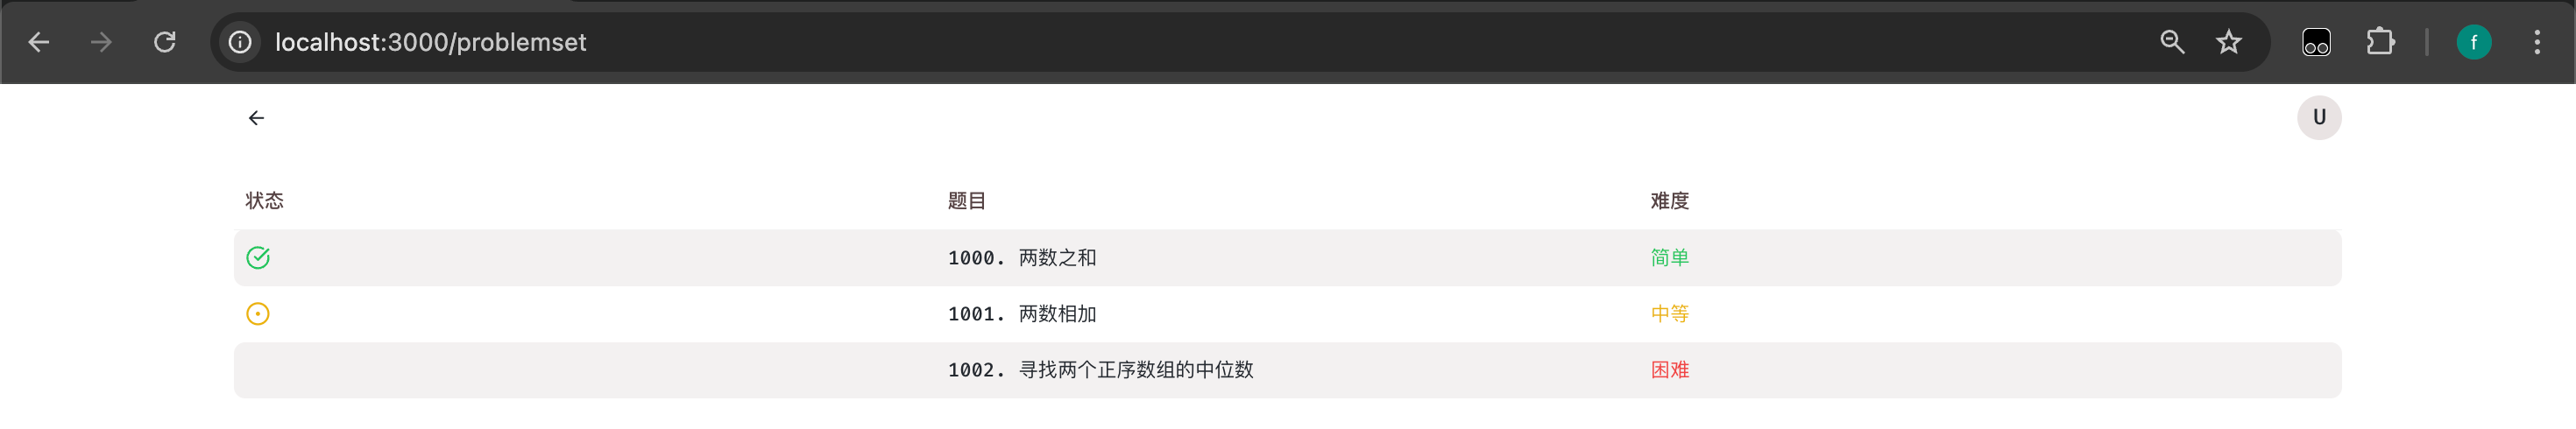
\includegraphics[width=0.78\textwidth]{images/fig6-2.png}
  \caption{题目列表页面截图}
  \label{fig:ch6-problemlist}
\end{figure}

当前工程实现与构建结果表明，系统主线功能已经基本齐备。用户注册登录、题目访问、模板加载、代码提交、结果查看和 AI 反馈展示等操作均可正常完成。与此同时，项目也通过了 \texttt{bun run lint} 与 \texttt{bun run build}，说明当前代码版本在静态检查和生产构建层面不存在明显阻塞问题。综合上述功能用例与构建结果，系统核心流程已具备稳定演示能力。

\section{判题正确性验证}

判题正确性测试是本系统测试中的核心部分，重点在于确认系统能否准确识别不同提交结果类型。本文围绕代表性题目构造了正确程序、编译错误程序、答案错误程序、运行错误程序以及时间超限程序等样例，并对系统返回状态进行逐项核对。对于输出比对相关逻辑，本文同时确认裁剪配置不会破坏结果判定的一致性。

在此处，关键并非题目数量，而是核心状态能否均被准确识别。基于此，本文运用状态覆盖优先的测试方式：围绕一个输入输出比较清晰的代表性题目，分别建立 \texttt{AC}、\texttt{CE}、\texttt{WA}、\texttt{RE}、\texttt{TLE} 等样例，并且逐一核对系统返回的结果。如此一来，更易于说明系统是否具备基本可靠的判题能力。

\begingroup
\small
\setlength{\LTleft}{\fill}
\setlength{\LTright}{\fill}
\setlength{\tabcolsep}{2pt}
\begin{xltabular}{\textwidth}{
P{0.07\textwidth}
P{0.10\textwidth}
>{\hsize=1.20\hsize\RaggedRight\arraybackslash}X
P{0.10\textwidth}
P{0.11\textwidth}
P{0.09\textwidth}
>{\hsize=1.10\hsize\RaggedRight\arraybackslash}X
}
\caption{判题正确性测试结果}\label{tab:ch6-judge-correctness}\\
\toprule
编号 & 测试类型 & 输入代码特征 & 预期状态 & 实际状态 & 是否通过 & 备注 \\
\midrule
\endfirsthead
\multicolumn{7}{c}{续表\thetable}\\
\toprule
编号 & 测试类型 & 输入代码特征 & 预期状态 & 实际状态 & 是否通过 & 备注 \\
\midrule
\endhead
\bottomrule
\endfoot
J-01 & 正确程序 & 全用例可过 & AC & AC & 通过 & 图~\ref{fig:ch5-submit} \\
J-02 & 编译错误程序 & 缺分号等 & CE & CE & 通过 & 图~\ref{fig:ch5-submission-list} \\
J-03 & 答案错误程序 & 输出与标答不符 & WA & WA & 通过 & 图~\ref{fig:ch5-submission-list} \\
J-04 & 运行错误程序 & 运行期异常退出 & RE & RE & 通过 & \texttt{abort()}；图~\ref{fig:ch5-submission-list} \\
J-05 & 时间超限程序 & 死循环/长期无响应 & TLE & TLE & 通过 & 图~\ref{fig:ch5-submission-list} \\
\bottomrule
\end{xltabular}
\endgroup

\begingroup
\small
\setlength{\LTleft}{\fill}
\setlength{\LTright}{\fill}
\setlength{\tabcolsep}{2pt}
\begin{xltabular}{\textwidth}{
P{0.07\textwidth}
P{0.11\textwidth}
>{\hsize=1.00\hsize\RaggedRight\arraybackslash}X
>{\hsize=1.10\hsize\RaggedRight\arraybackslash}X
>{\hsize=1.20\hsize\RaggedRight\arraybackslash}X
}
\caption{不同错误类型样例与系统返回状态}\label{tab:ch6-error-samples}\\
\toprule
编号 & 错误类型 & 构造方式 & 页面表现 & 结果说明 \\
\midrule
\endfirsthead
\multicolumn{5}{c}{续表\thetable}\\
\toprule
编号 & 错误类型 & 构造方式 & 页面表现 & 结果说明 \\
\midrule
\endhead
\bottomrule
\endfoot
E-01 & 编译错误 & 删分号/未声明变量等 & 返回 CE 并展示编译信息 & 语法层失败可识别 \\
E-02 & 答案错误 & 固定错答或漏分支 & 返回 WA 并保留用例信息 & 标答比对可用 \\
E-03 & 运行错误 & \texttt{abort()} 等 & 返回 RE & 运行期异常可识别 \\
E-04 & 时间超限 & \texttt{while(1)\{\}} & 返回 TLE & 时限控制可用 \\
\bottomrule
\end{xltabular}
\endgroup

判题正确性是本系统最核心的验证内容，实际测试表明，系统在接收到提交后，能够依次完成前置校验、编译、运行和结果判定，并对 \texttt{AC}、\texttt{CE}、\texttt{WA}、\texttt{RE} 和 \texttt{TLE} 等核心状态给出与预期一致的返回结果。这说明系统已具备基本可靠的判题能力。针对容器清理、远程 Docker 连接与输出记录等边界条件，本文在异常路径中给出状态回写与日志追踪策略\cite{alemu2023serverless,kubernetesdocs}。

\section{安全隔离与恶意代码防护验证}

除常规判题状态验证之外，本文还补充了高风险样例来检验隔离边界。测试重点覆盖三类行为：进程滥用、内存滥用、网络外联。并且这些样例全部走与普通提交一致的默认判题链路，不额外增加特权配置，这样才能更真实地验证沙箱默认策略是否足够有效。

\begingroup
\small
\setlength{\LTleft}{\fill}
\setlength{\LTright}{\fill}
\setlength{\tabcolsep}{2pt}
\begin{xltabular}{\textwidth}{
P{0.08\textwidth}
P{0.16\textwidth}
>{\hsize=1.00\hsize\RaggedRight\arraybackslash}X
P{0.14\textwidth}
>{\hsize=1.30\hsize\RaggedRight\arraybackslash}X
}
\caption{恶意代码防护验证结果}\label{tab:ch6-security-cases}\\
\toprule
编号 & 攻击场景 & 样例行为 & 实际状态 & 验证结论 \\
\midrule
\endfirsthead
\multicolumn{5}{c}{续表\thetable}\\
\toprule
编号 & 攻击场景 & 样例行为 & 实际状态 & 验证结论 \\
\midrule
\endhead
\bottomrule
\endfoot
S-01 & 进程滥用 & 循环 \texttt{fork()} & TLE/RE & 容器内终止，未拖垮宿主 \\
S-02 & 内存滥用 & 超大连续申请 & MLE & 内存上限生效 \\
S-03 & 网络外联 & 容器内连公网 & RE & 默认网络隔离生效 \\
\bottomrule
\end{xltabular}
\endgroup

上述结果表明，平台当前的判题沙箱不仅能够处理普通错误类型，也能对高风险样例形成有效约束。对应样例代码见附录中的恶意代码样例，便于复核与复现实验。

\begin{figure}[htbp]
  \centering
  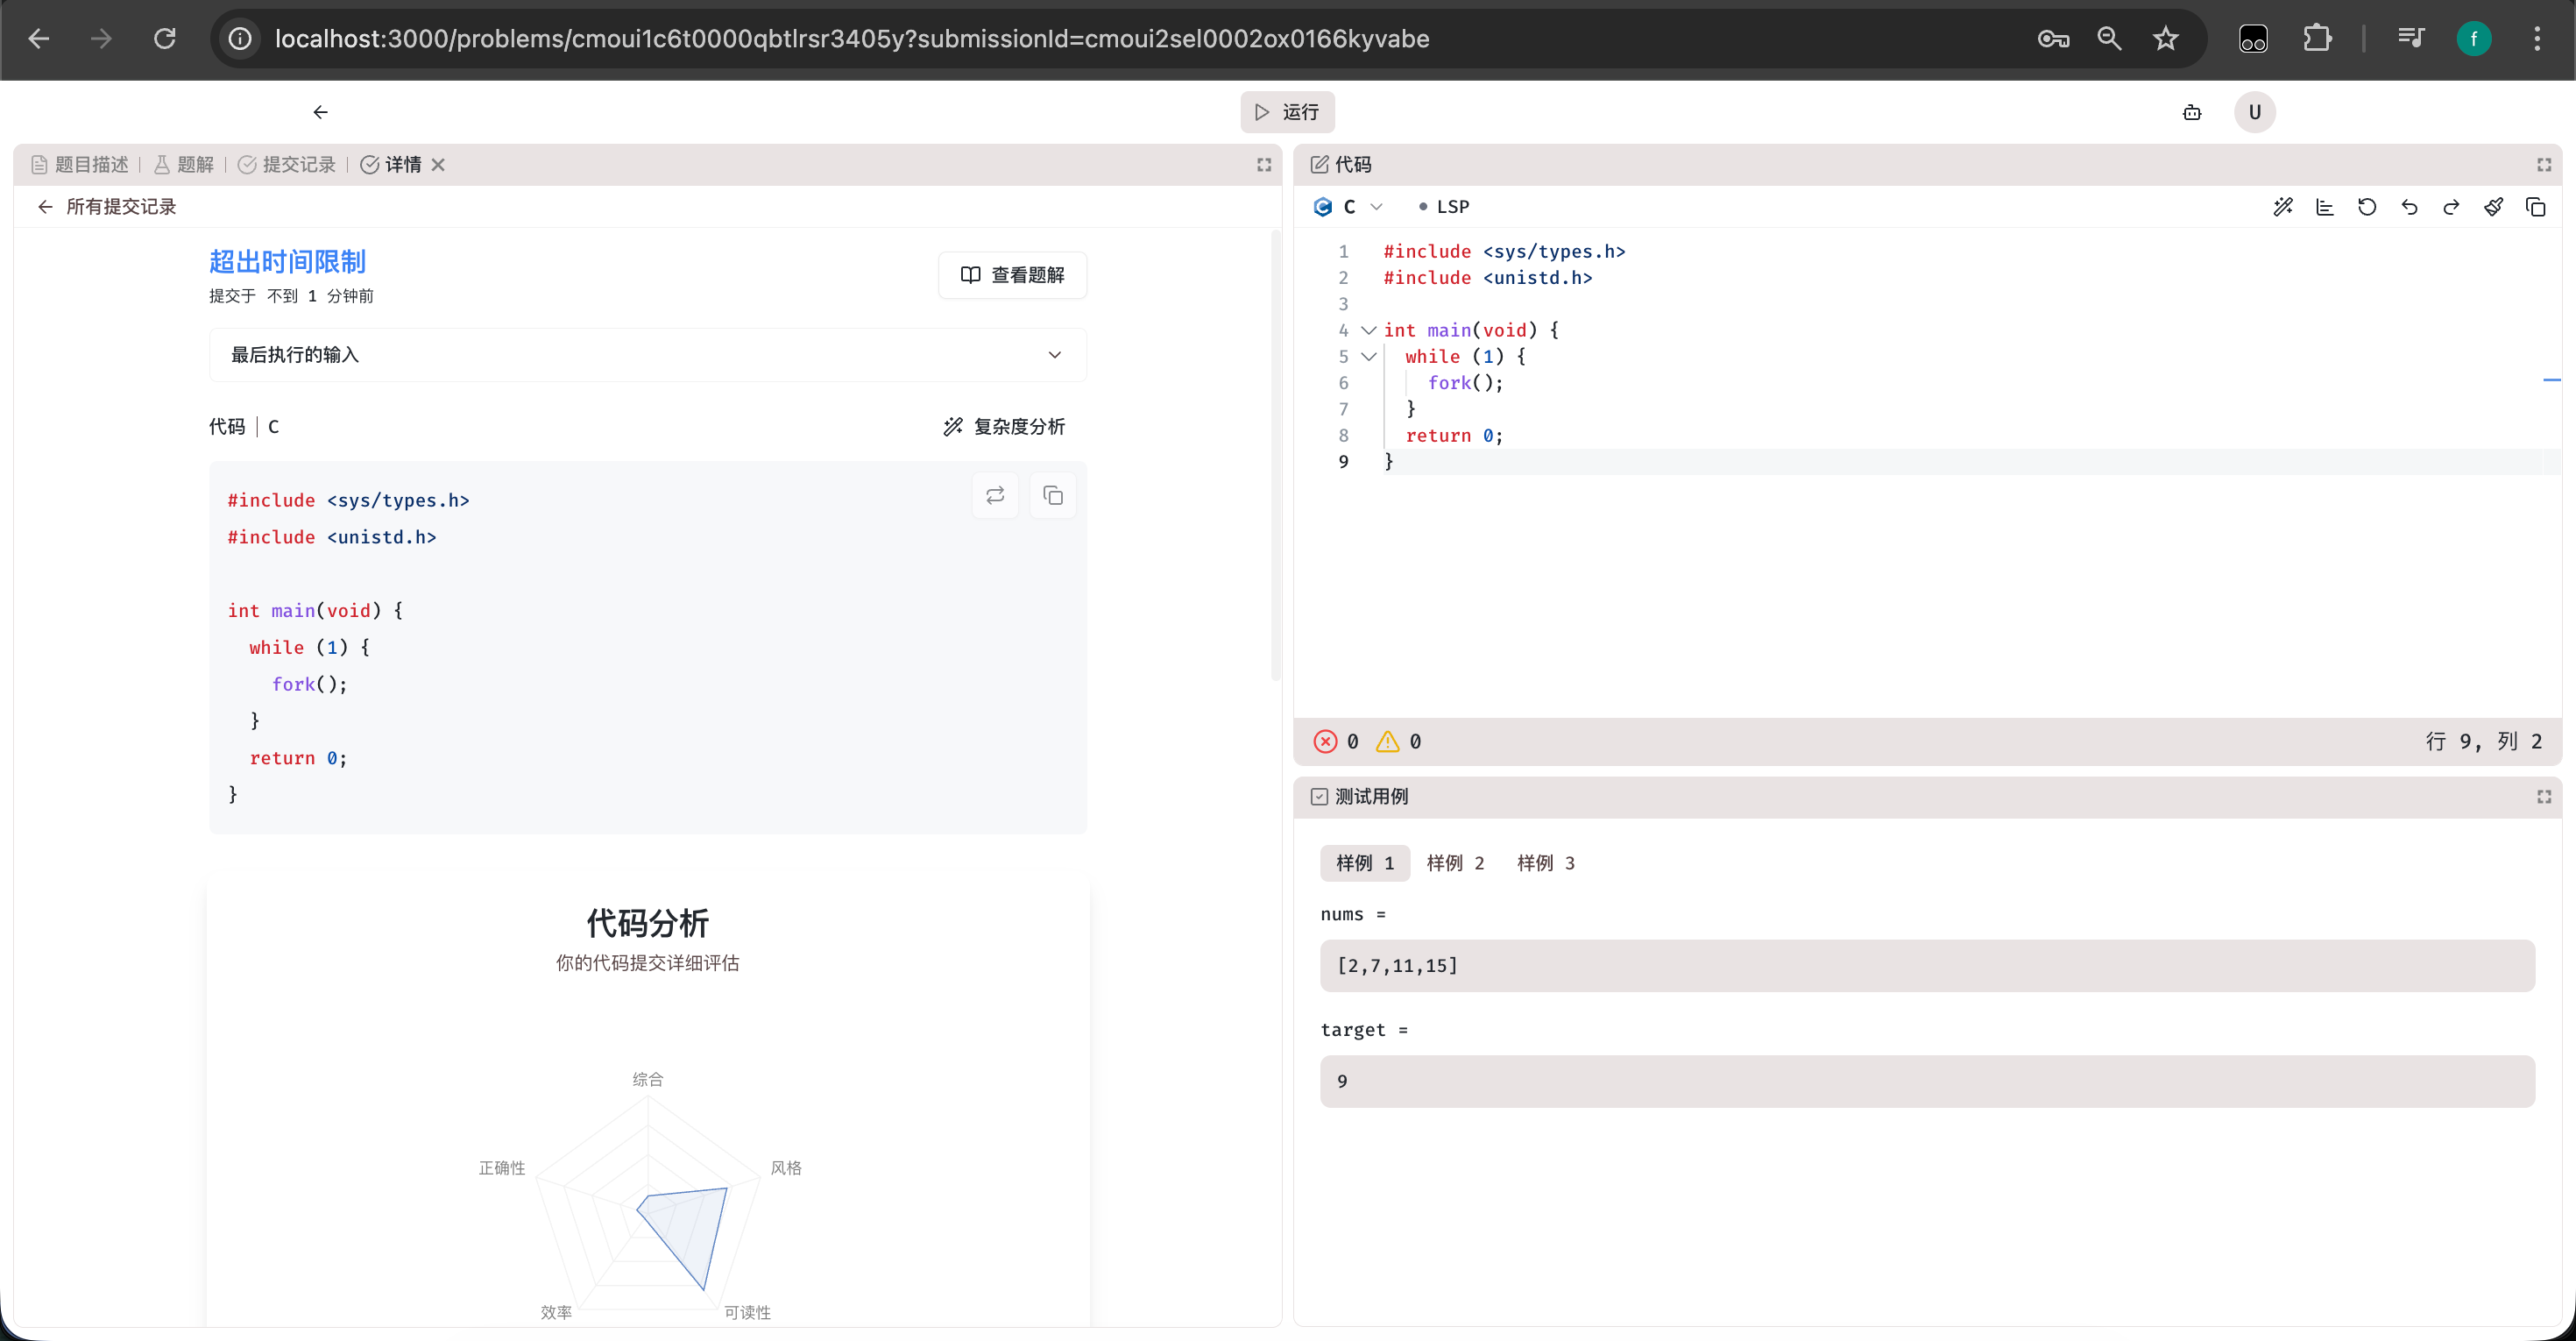
\includegraphics[width=0.92\textwidth]{images/fig6-10.png}
  \caption{进程滥用样例提交结果截图}
  \label{fig:ch6-security-fork}
\end{figure}

\begin{figure}[htbp]
  \centering
  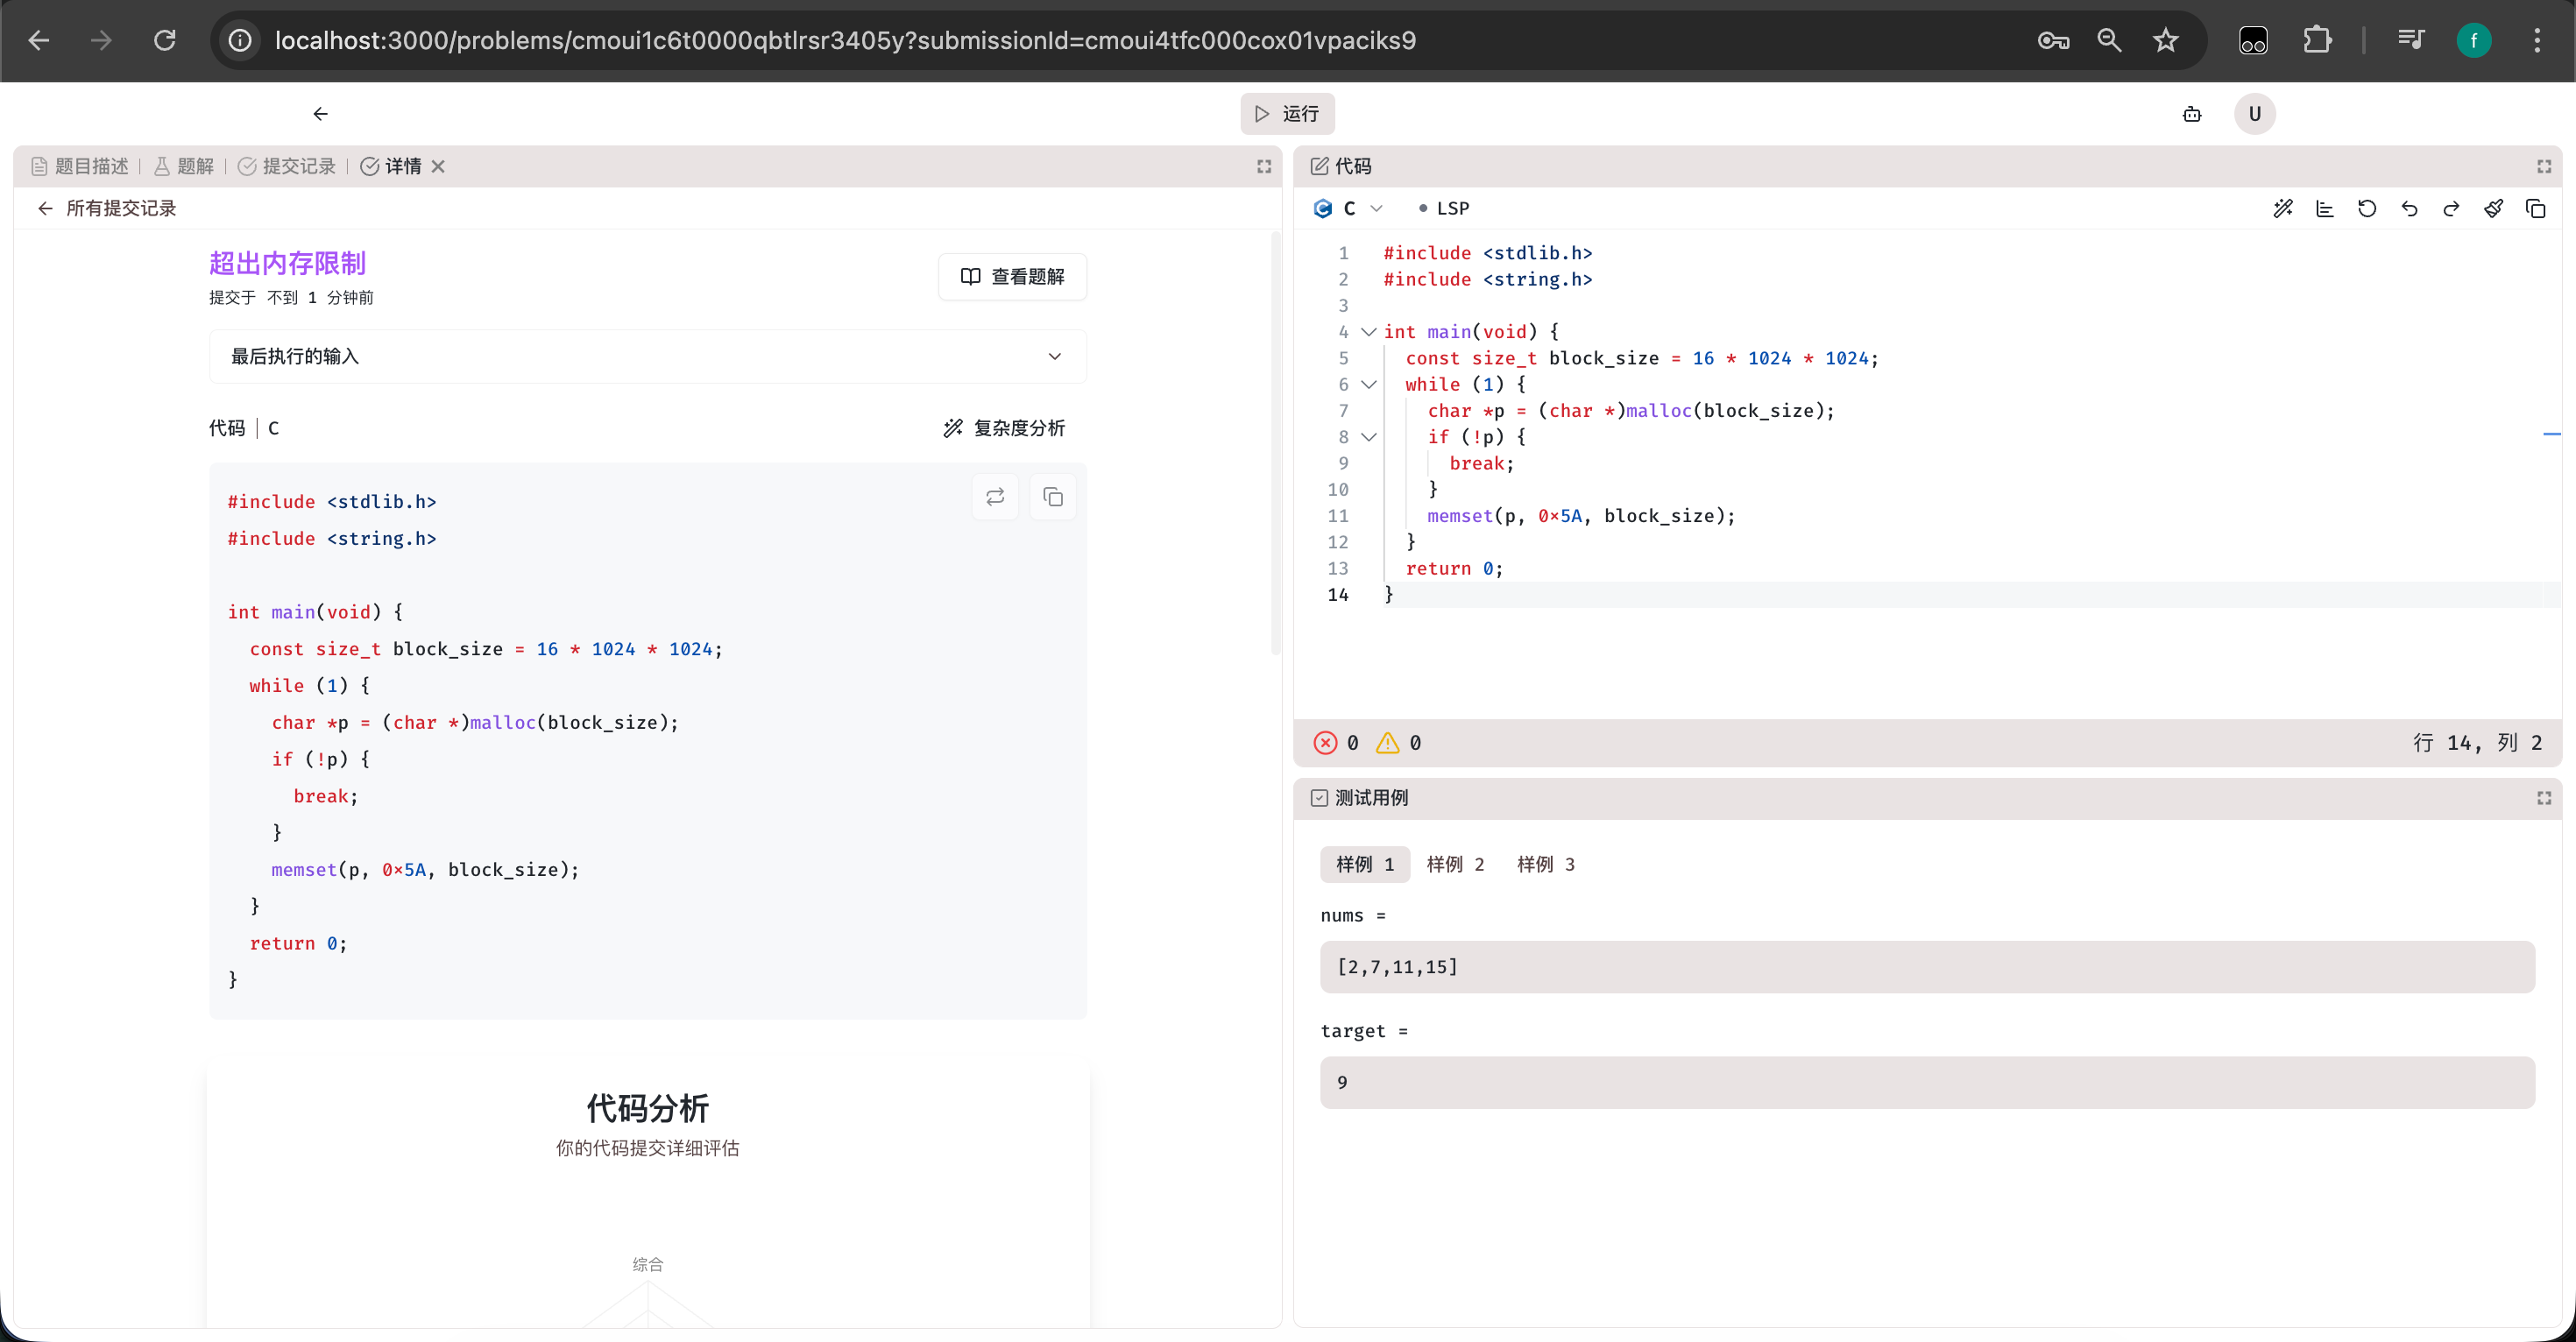
\includegraphics[width=0.92\textwidth]{images/fig6-11.png}
  \caption{内存滥用样例提交结果截图}
  \label{fig:ch6-security-memory}
\end{figure}

\begin{figure}[htbp]
  \centering
  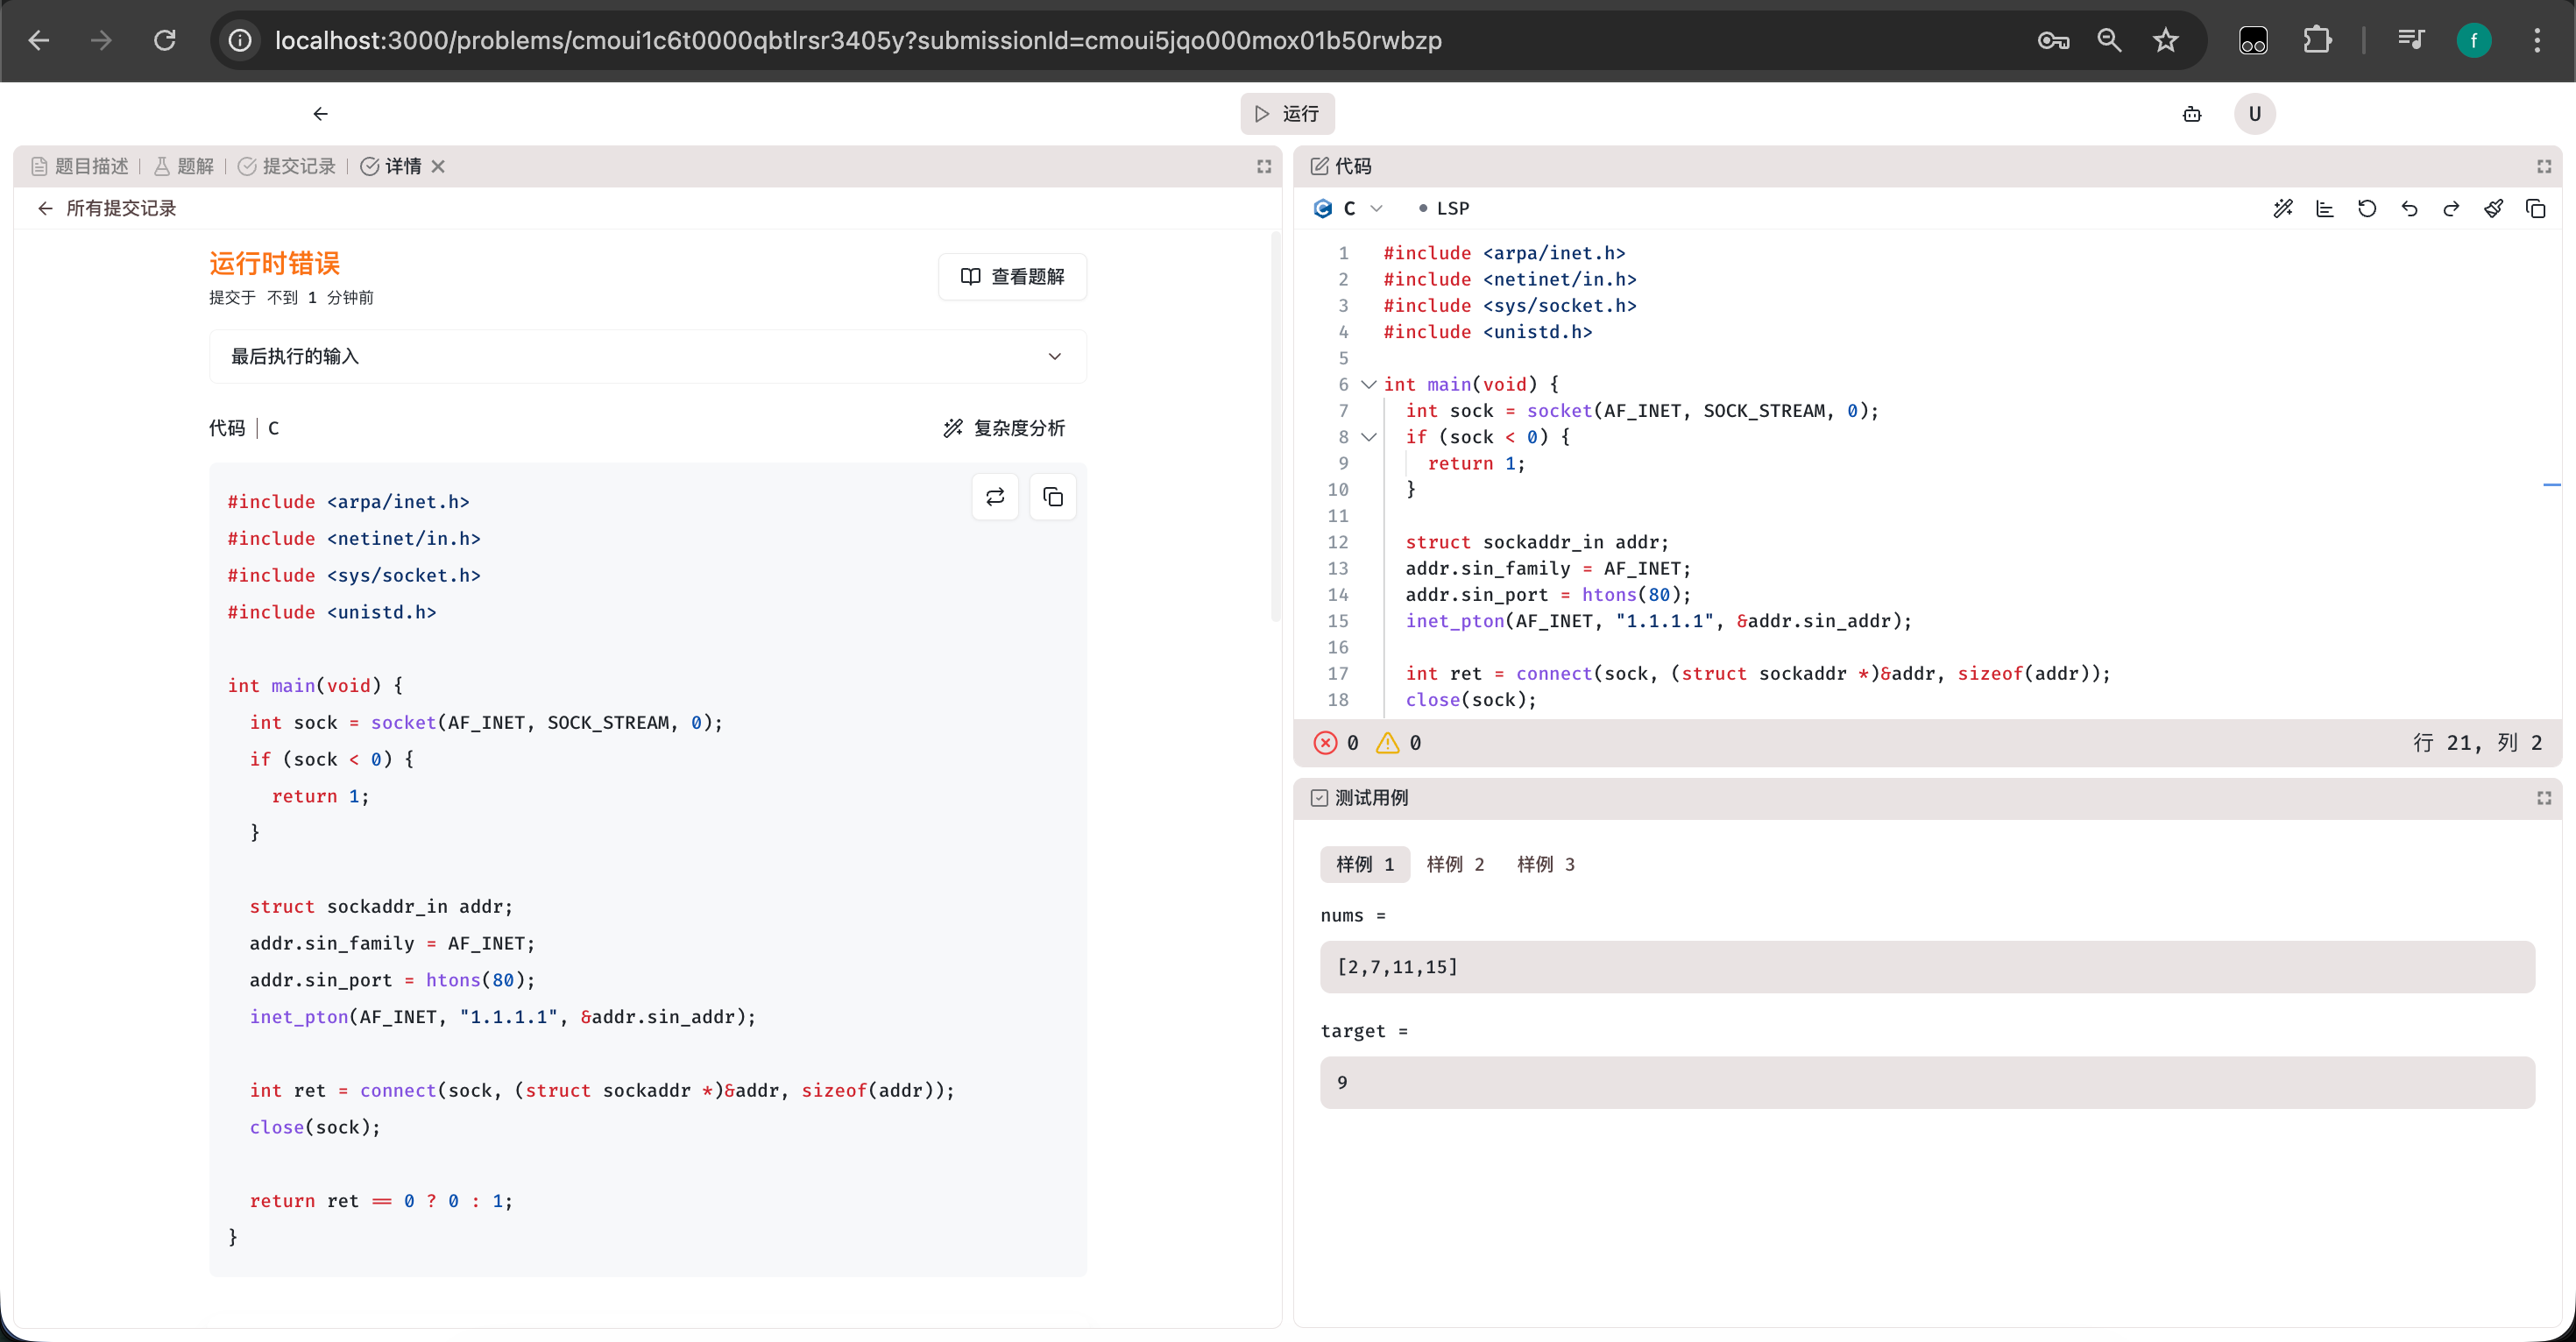
\includegraphics[width=0.92\textwidth]{images/fig6-12.png}
  \caption{网络外联样例提交结果截图}
  \label{fig:ch6-security-network}
\end{figure}

图~\ref{fig:ch6-security-fork}、图~\ref{fig:ch6-security-memory} 与图~\ref{fig:ch6-security-network} 分别对应进程滥用、内存滥用和网络外联三类场景。页面结果与表~\ref{tab:ch6-security-cases} 中的状态记录一致，能够直接展示平台在默认判题链路下对恶意行为的约束效果。

\section{AI 辅助反馈效果验证}

AI 辅助反馈效果分析选择了若干具有代表性的提交样例，例如编译错误、逻辑错误、低效实现和风格较差的代码，用于观察系统输出的复杂度估计、评分结果和反馈内容是否具有合理性。该部分测试的关注重点不是 AI 是否绝对正确，而是其输出是否与客观判题结果一致、是否具有解释价值、是否避免直接给出完整答案以及是否能够帮助学生理解问题。

\begingroup
\small
\setlength{\LTleft}{\fill}
\setlength{\LTright}{\fill}
\setlength{\tabcolsep}{2pt}
\begin{xltabular}{\textwidth}{
P{0.07\textwidth}
P{0.13\textwidth}
>{\hsize=1.00\hsize\RaggedRight\arraybackslash}X
>{\hsize=1.10\hsize\RaggedRight\arraybackslash}X
>{\hsize=1.00\hsize\RaggedRight\arraybackslash}X
>{\hsize=0.90\hsize\RaggedRight\arraybackslash}X
}
\caption{AI 辅助反馈效果示例}\label{tab:ch6-ai-feedback-cases}\\
\toprule
编号 & 提交场景 & AI 输出重点 & 预期评价维度 & 实际情况 & 展示价值 \\
\midrule
\endfirsthead
\multicolumn{6}{c}{续表\thetable}\\
\toprule
编号 & 提交场景 & AI 输出重点 & 预期评价维度 & 实际情况 & 展示价值 \\
\midrule
\endhead
\bottomrule
\endfoot
A-01 & 编译错误代码 & 原因/位置/修改提示 & 指语法问题、少代写 & 指出缺分号等 & 可用 \\
A-02 & 答案错误代码 & 逻辑/边界提示 & 解释 WA 主因 & 指出恒返 \texttt{[0,0]} & 可用；图~\ref{fig:ch6-ai-wa} \\
A-03 & 低效正确代码 & 复杂度与优化方向 & 复杂度合理 & \(O(N^2)\)/\(O(1)\)，建议哈希 & 可用；图~\ref{fig:ch5-ai-feedback} \\
A-04 & 可读性较差代码 & 命名/结构/风格 & 结构化意见 & 风格约 30、可读约 35 & 可用；图~\ref{fig:ch6-ai-readability} \\
\bottomrule
\end{xltabular}
\endgroup

\begin{figure}[htbp]
  \centering
  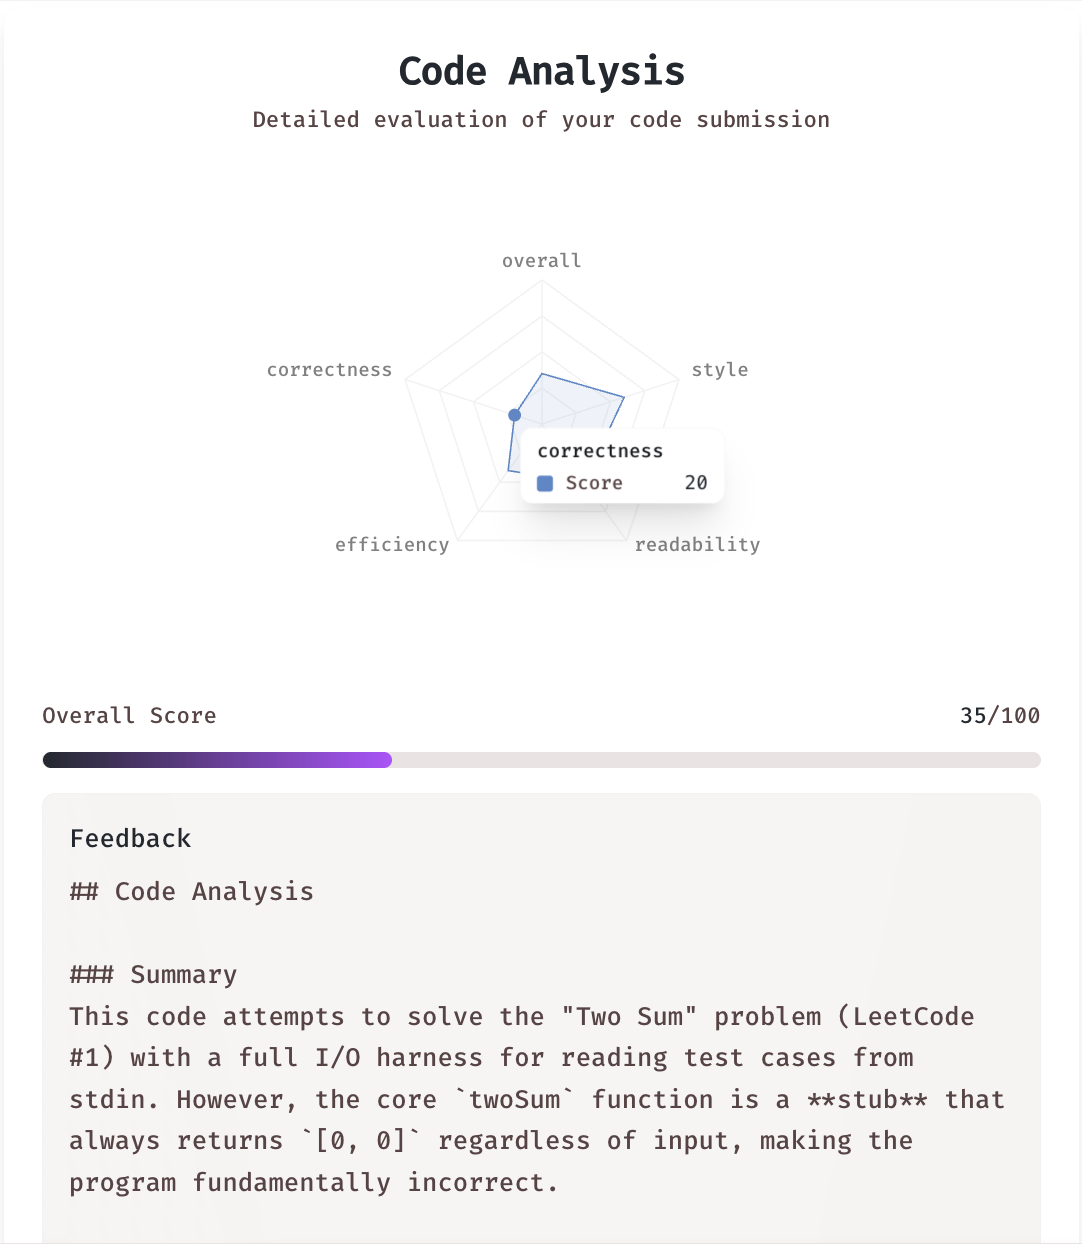
\includegraphics[width=0.72\textwidth]{images/fig6-1.png}
  \caption{答案错误代码的 AI 分析结果截图}
  \label{fig:ch6-ai-wa}
\end{figure}

\begin{figure}[htbp]
  \centering
  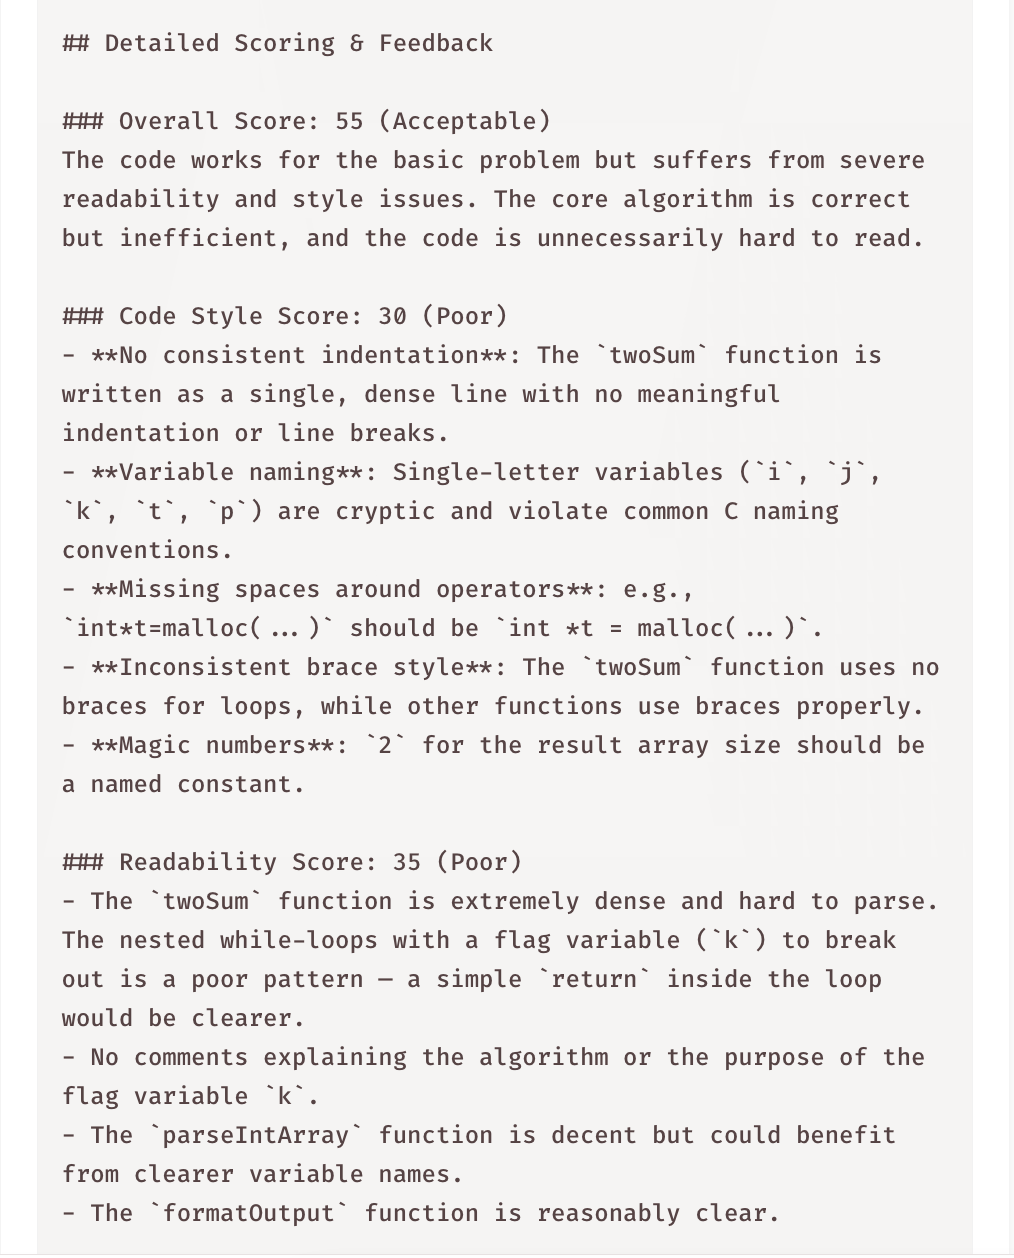
\includegraphics[width=0.72\textwidth]{images/fig6-3.png}
  \caption{可读性较差代码的 AI 分析结果截图}
  \label{fig:ch6-ai-readability}
\end{figure}

AI 辅助反馈部分作为客观判题之后的附加分析存在。从样例结果可见，AI 对编译错误、答案错误、低效正确代码和可读性较差代码都能给出与提交情形基本一致的解释和改进方向，说明该模块已经能够起到一定的学习支持作用，但它并不替代判题结果本身。

\section{工作区交互与多终端适配验证}

\begingroup
\small
\setlength{\LTleft}{\fill}
\setlength{\LTright}{\fill}
\setlength{\tabcolsep}{2pt}
\begin{xltabular}{\textwidth}{
P{0.07\textwidth}
P{0.16\textwidth}
P{0.12\textwidth}
>{\hsize=1.20\hsize\RaggedRight\arraybackslash}X
>{\hsize=0.90\hsize\RaggedRight\arraybackslash}X
}
\caption{界面与交互能力测试结果}\label{tab:ch6-interaction}\\
\toprule
编号 & 测试项 & 实际结果 & 结果说明 & 截图对应 \\
\midrule
\endfirsthead
\multicolumn{5}{c}{续表\thetable}\\
\toprule
编号 & 测试项 & 实际结果 & 结果说明 & 截图对应 \\
\midrule
\endhead
\bottomrule
\endfoot
I-01 & 响应式布局 & 通过 & 窄屏主流程可读 & 图~\ref{fig:mobile-workspace} \\
I-02 & 多语言切换 & 通过 & 界面与题面语种一致 & 图~\ref{fig:lang-switch} \\
I-03 & 深浅色主题 & 通过 & 页/工作区/代码区配色一致 & 图~\ref{fig:dark-theme-workspace} \\
I-04 & 编辑器 AI 工具栏 & 通过 & Diff 可看改动，未静默覆盖 & 图~\ref{fig:diff-view} \\
I-05 & 机器人问答面板 & 通过 & 回答绑定当前代码上下文 & 图~\ref{fig:ai-chat-panel} \\
I-06 & 语言服务 LSP 体验 & 通过 & 连接态可见；错误可出诊断 & 图~\ref{fig:ch6-lsp} \\
\bottomrule
\end{xltabular}
\endgroup

\begin{figure}[htbp]
  \centering
  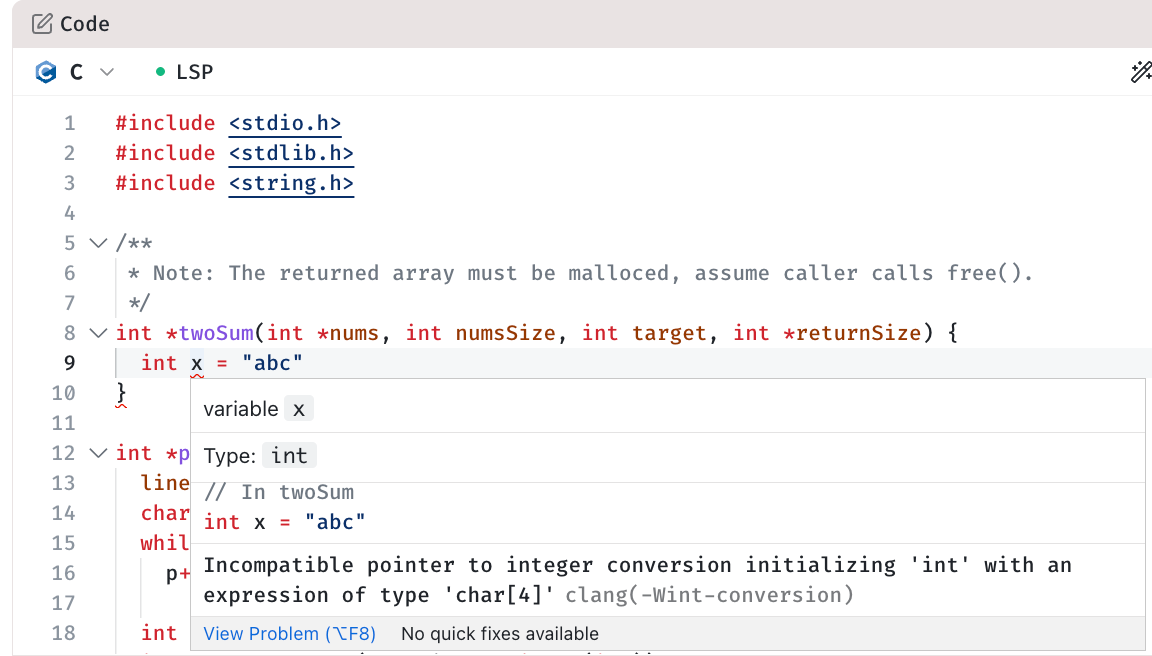
\includegraphics[width=0.92\linewidth]{images/fig6-9.png}
  \caption{LSP 连接指示与编辑器诊断标记同屏截图}
  \label{fig:ch6-lsp}
\end{figure}

\begin{figure}[htbp]
  \centering
  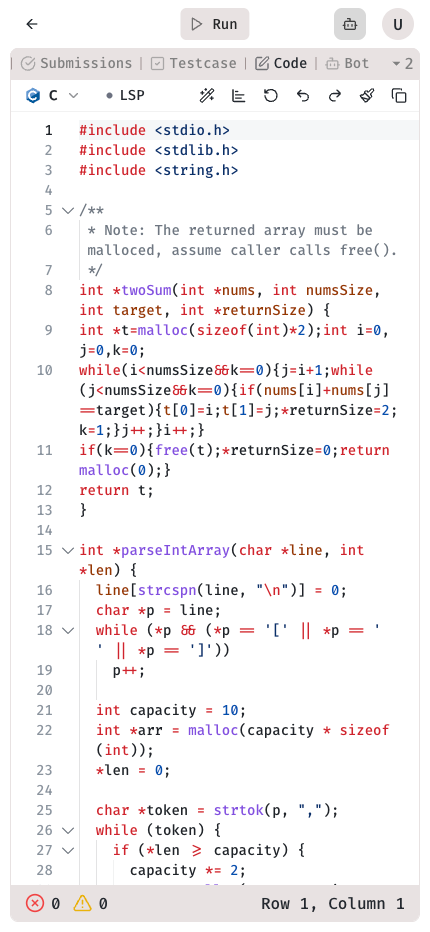
\includegraphics[width=0.30\textwidth]{images/fig6-4.png}
  \caption{移动端题目工作区截图}
  \label{fig:mobile-workspace}
\end{figure}

\begin{figure}[htbp]
  \centering
  \begin{subfigure}{0.49\textwidth}
    \centering
    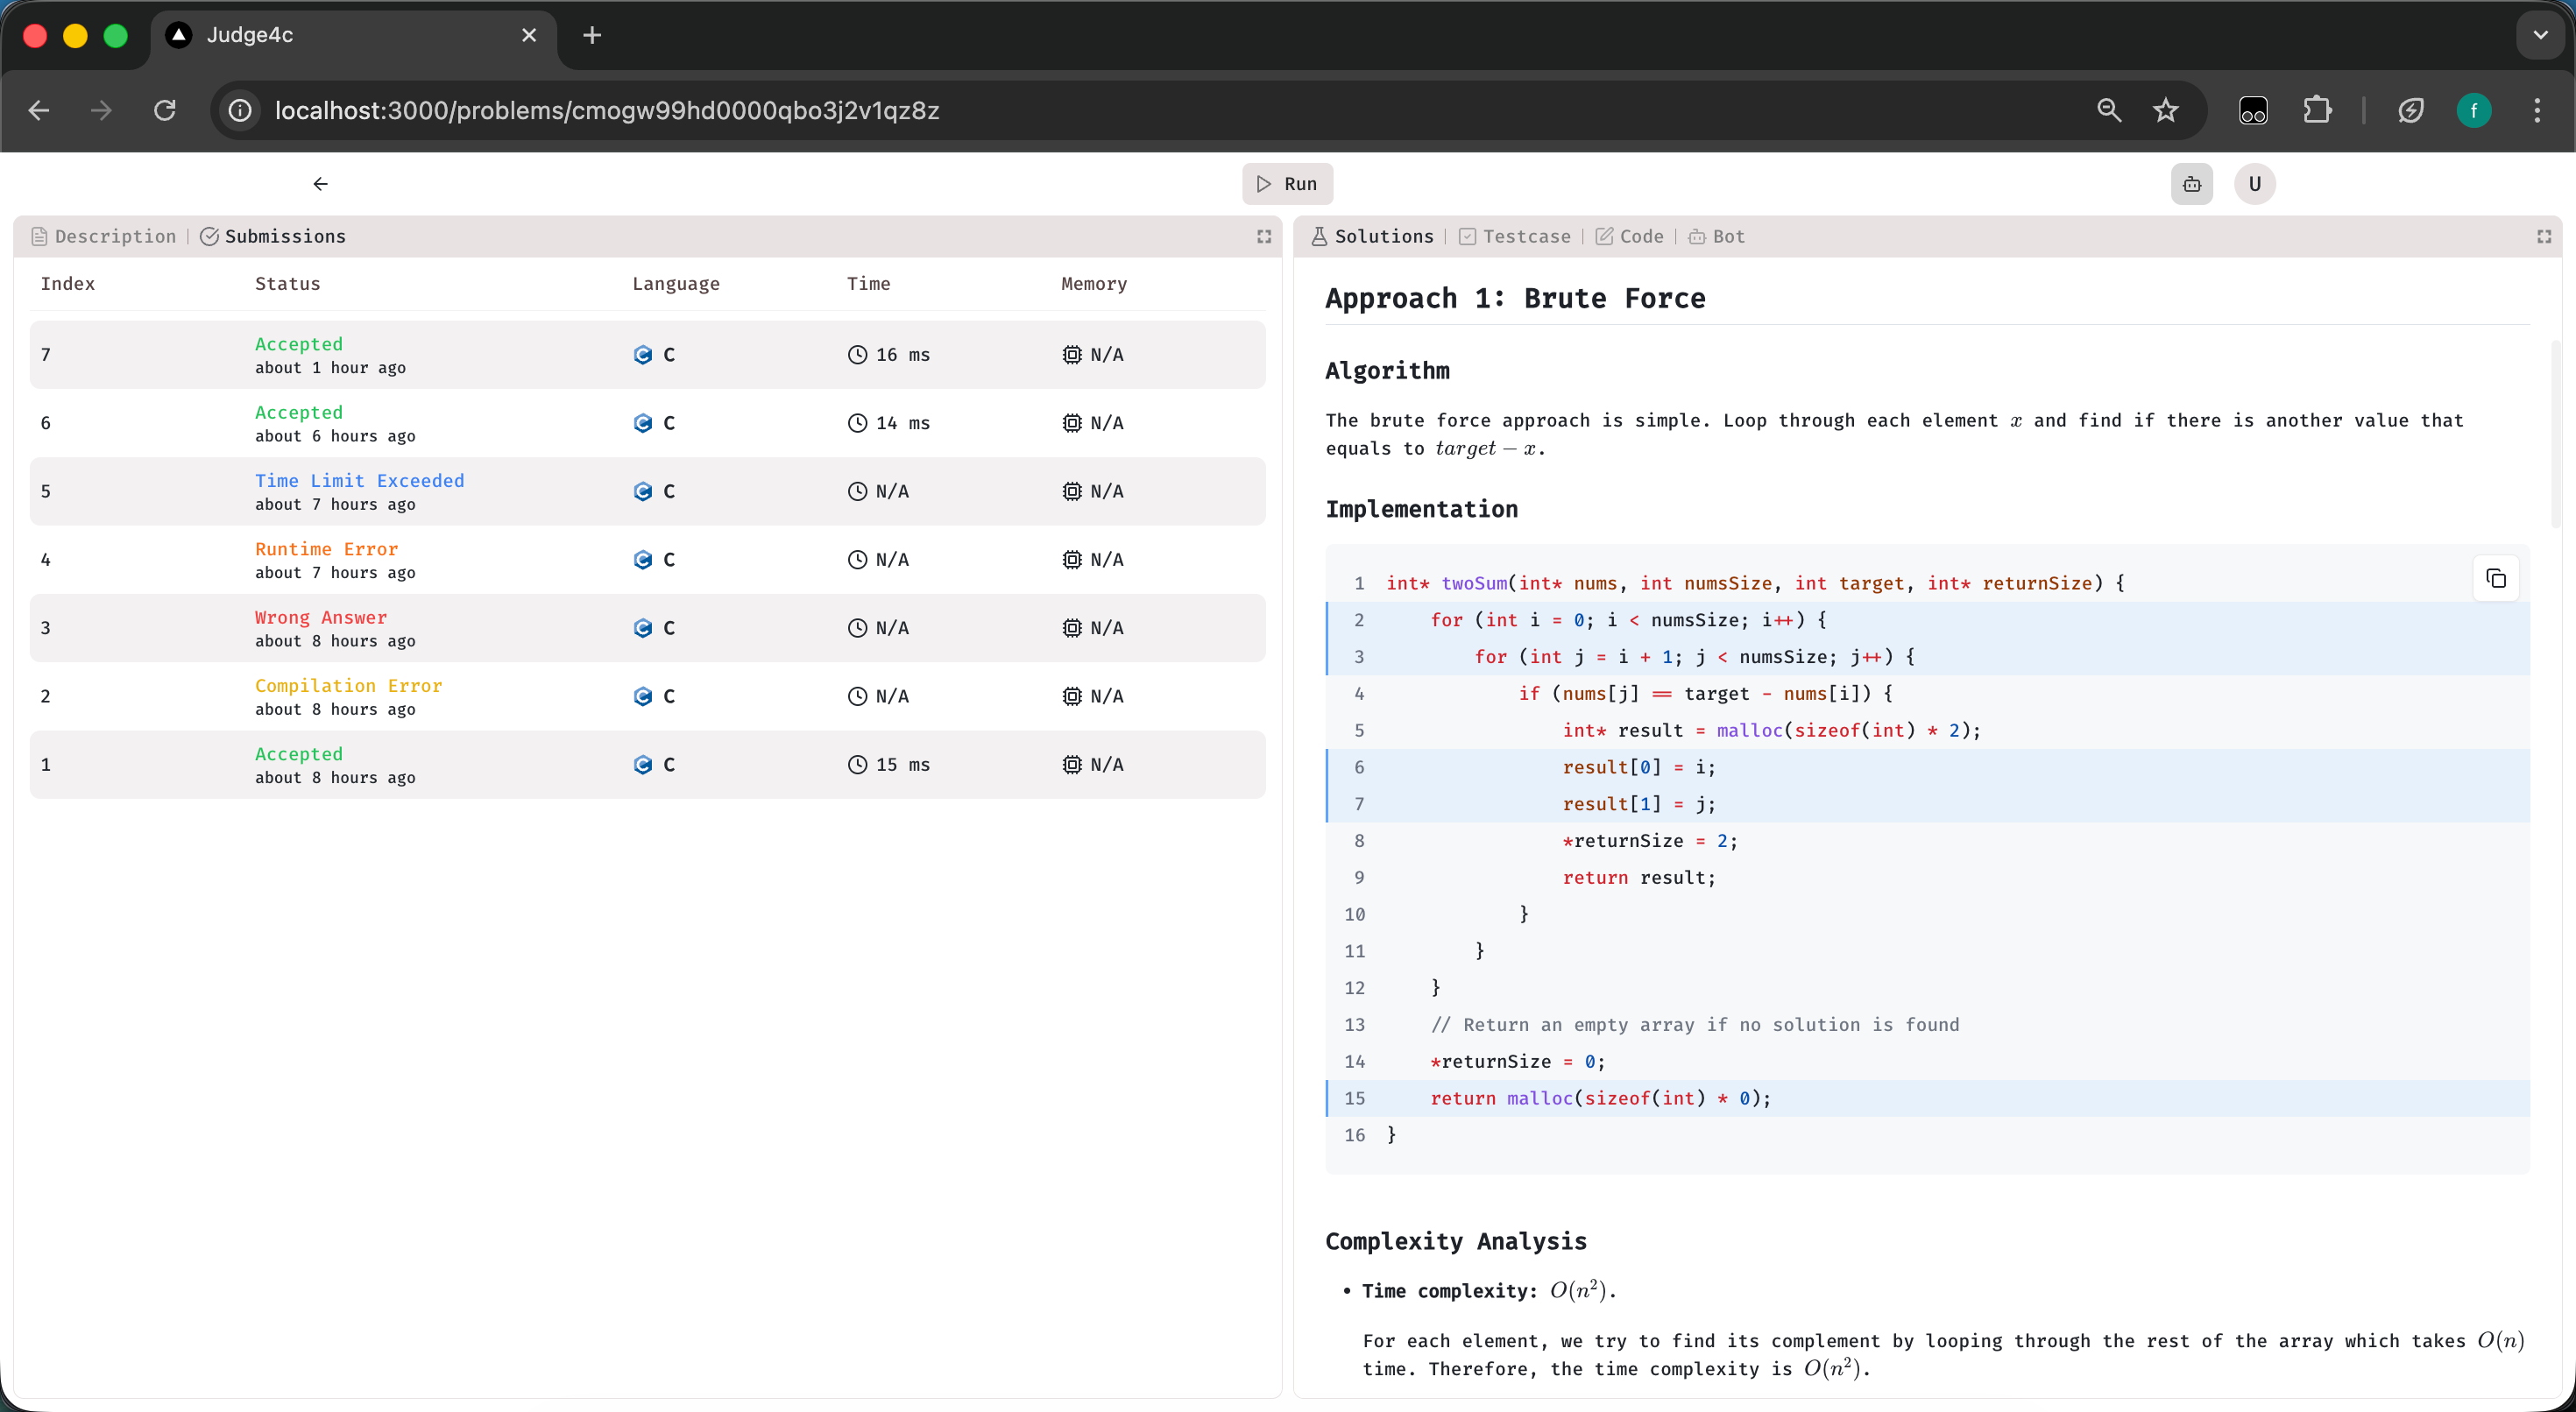
\includegraphics[width=\textwidth]{images/fig6-5a.png}
    \caption{英文界面与题面内容}
  \end{subfigure}
  \hfill
  \begin{subfigure}{0.49\textwidth}
    \centering
    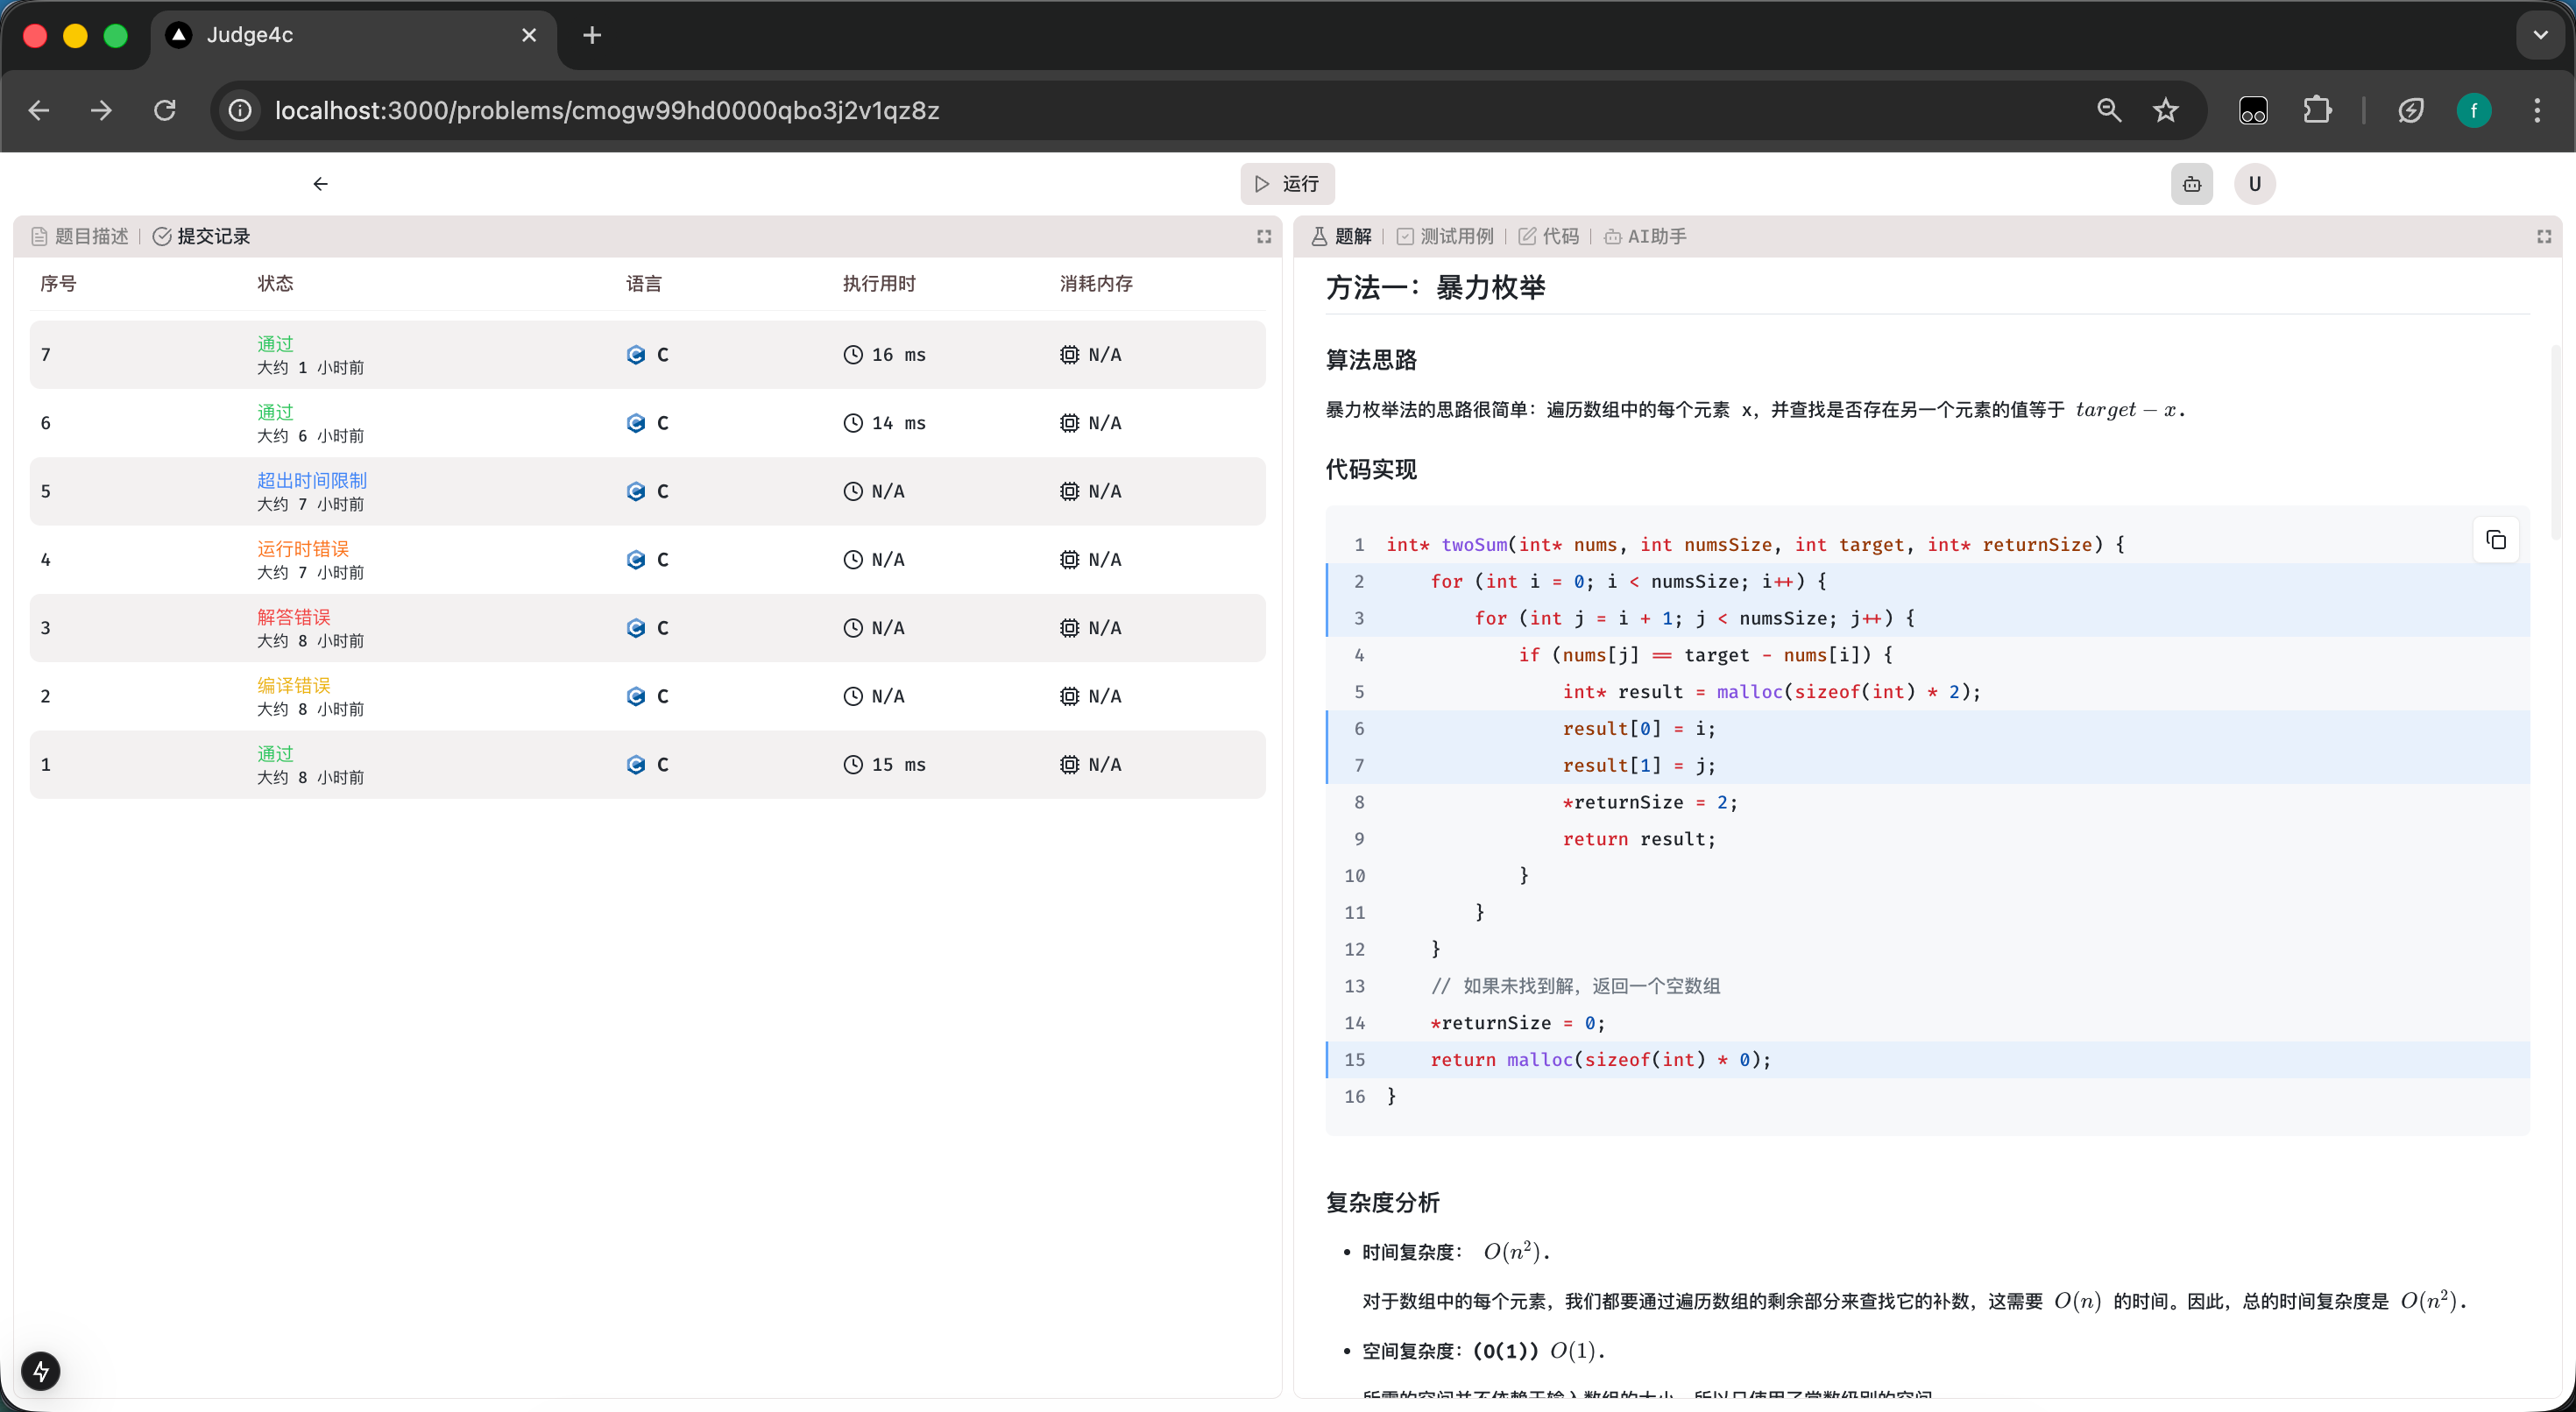
\includegraphics[width=\textwidth]{images/fig6-5b.png}
    \caption{中文界面与题面内容}
  \end{subfigure}
  \caption{中英文界面切换效果截图}
  \label{fig:lang-switch}
\end{figure}

\begin{figure}[htbp]
  \centering
  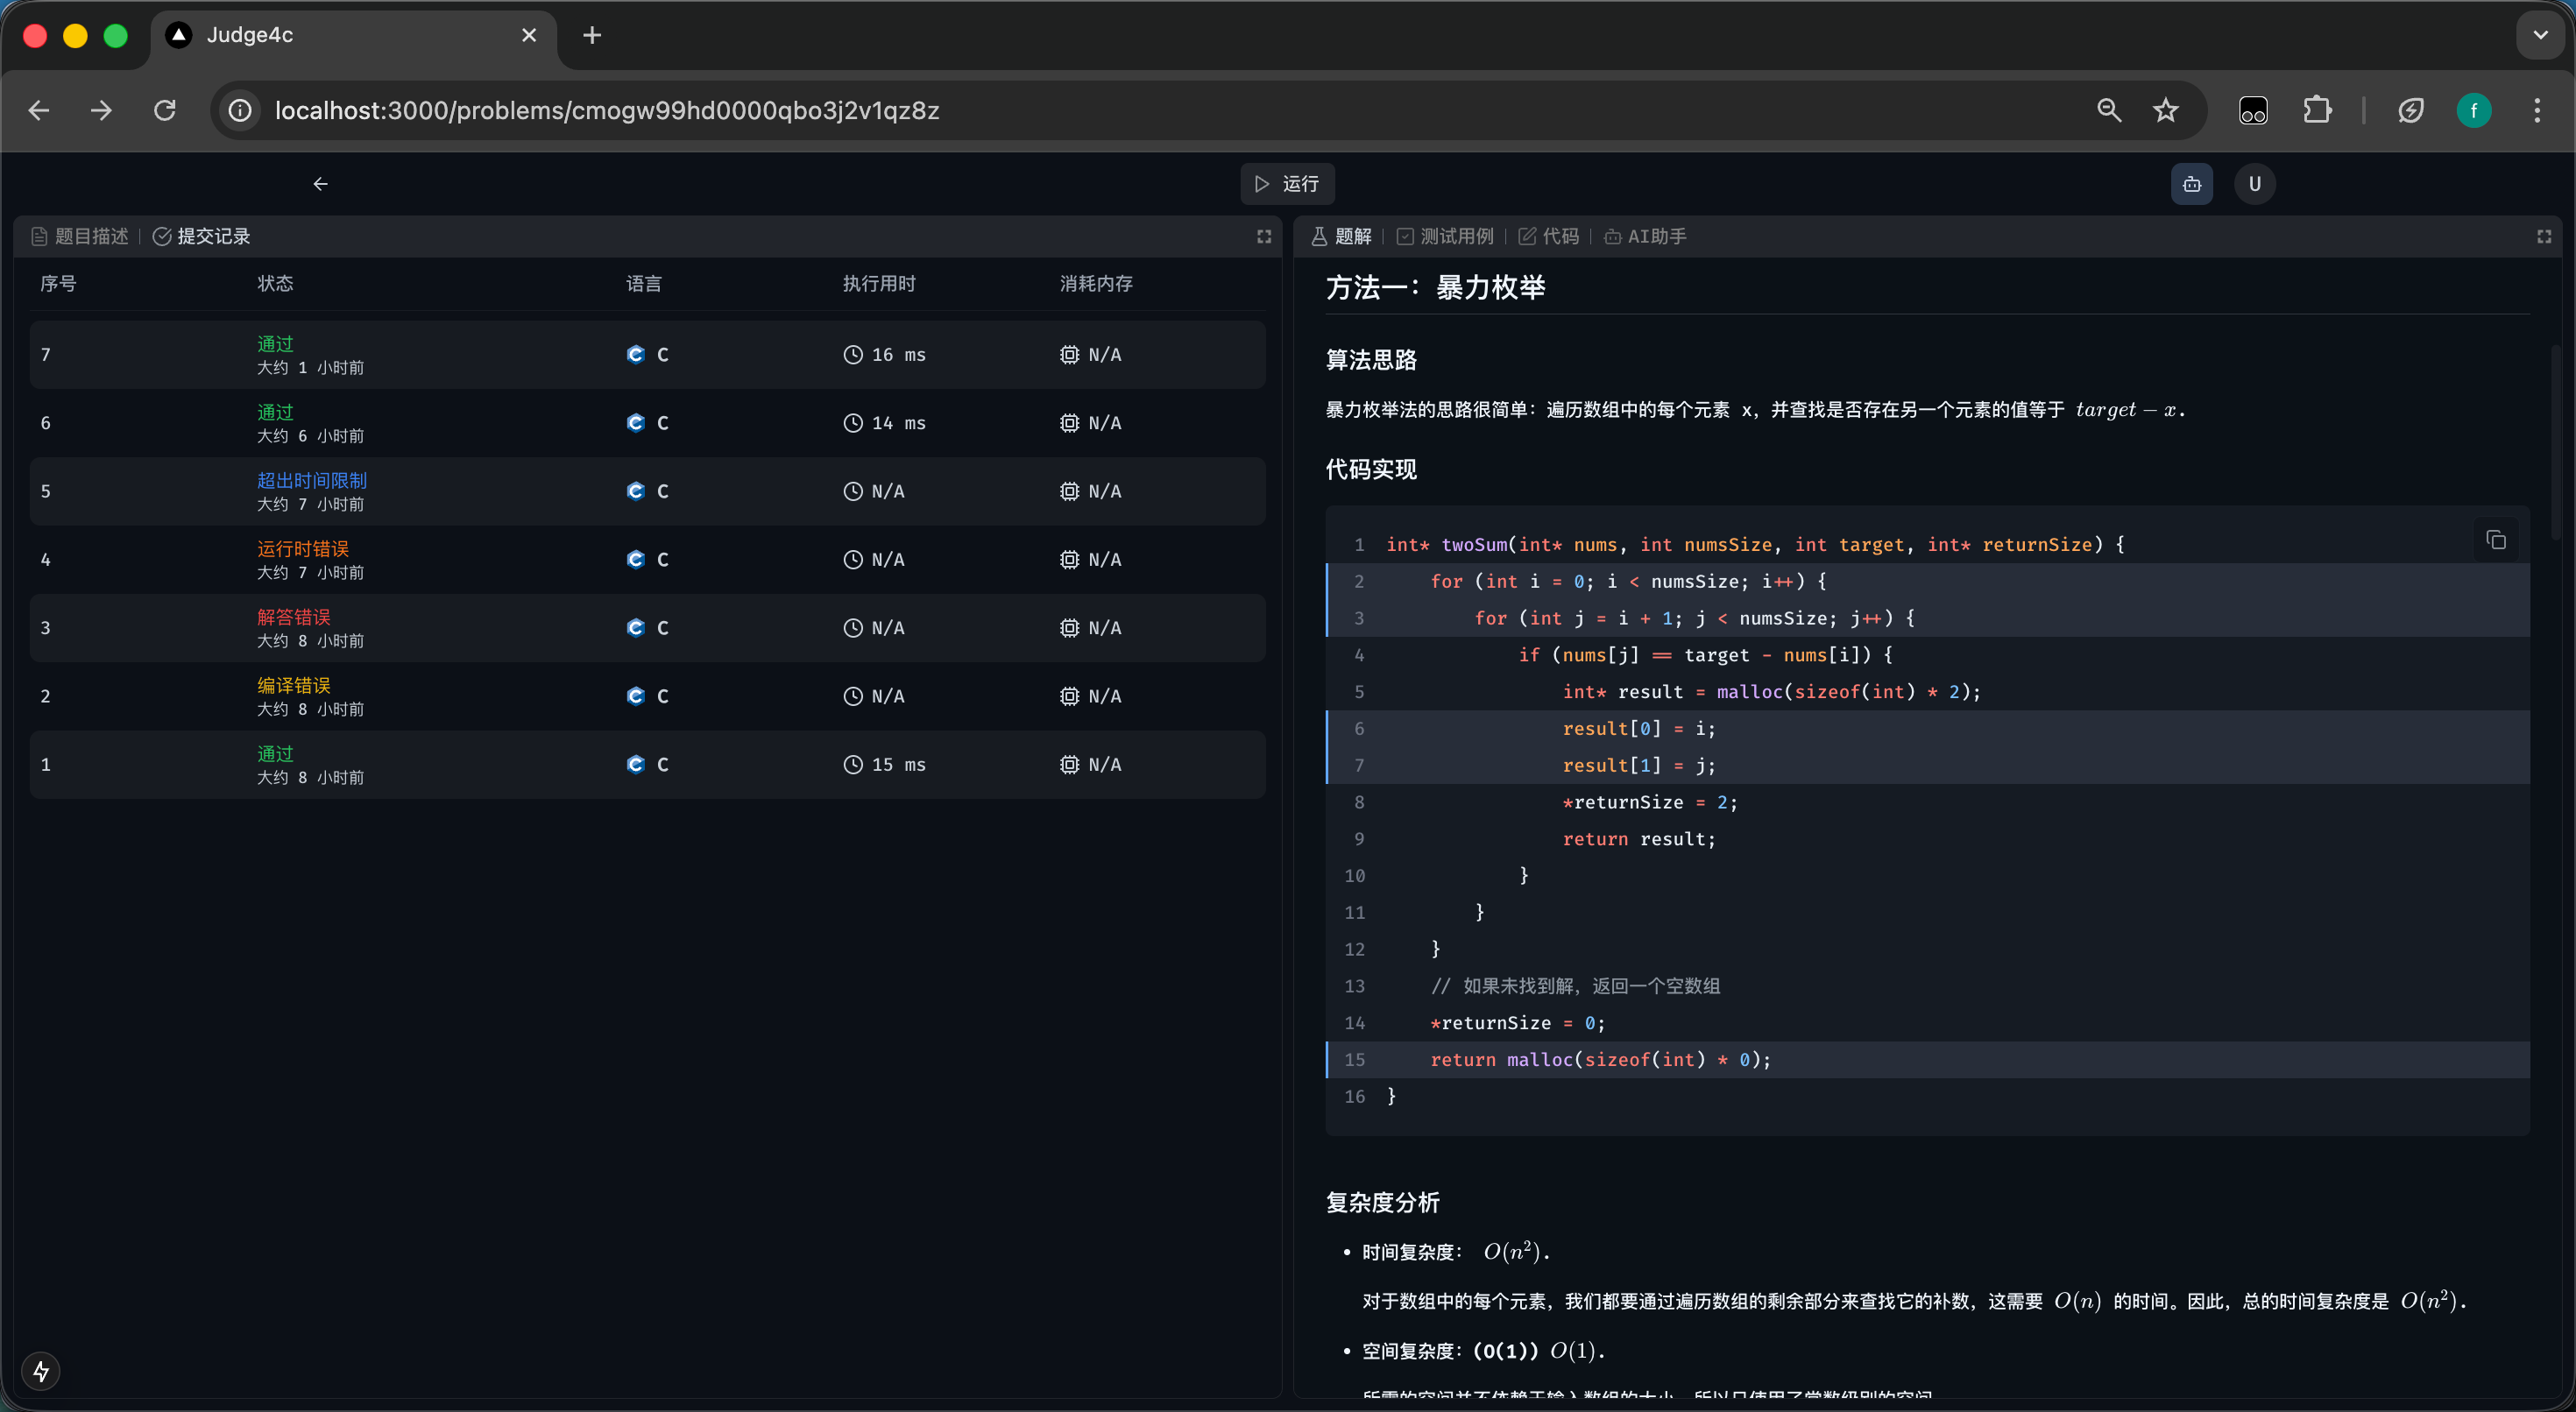
\includegraphics[width=0.96\textwidth]{images/fig6-6.png}
  \caption{深色主题下的题目工作区截图}
  \label{fig:dark-theme-workspace}
\end{figure}

\begin{figure}[htbp]
  \centering
  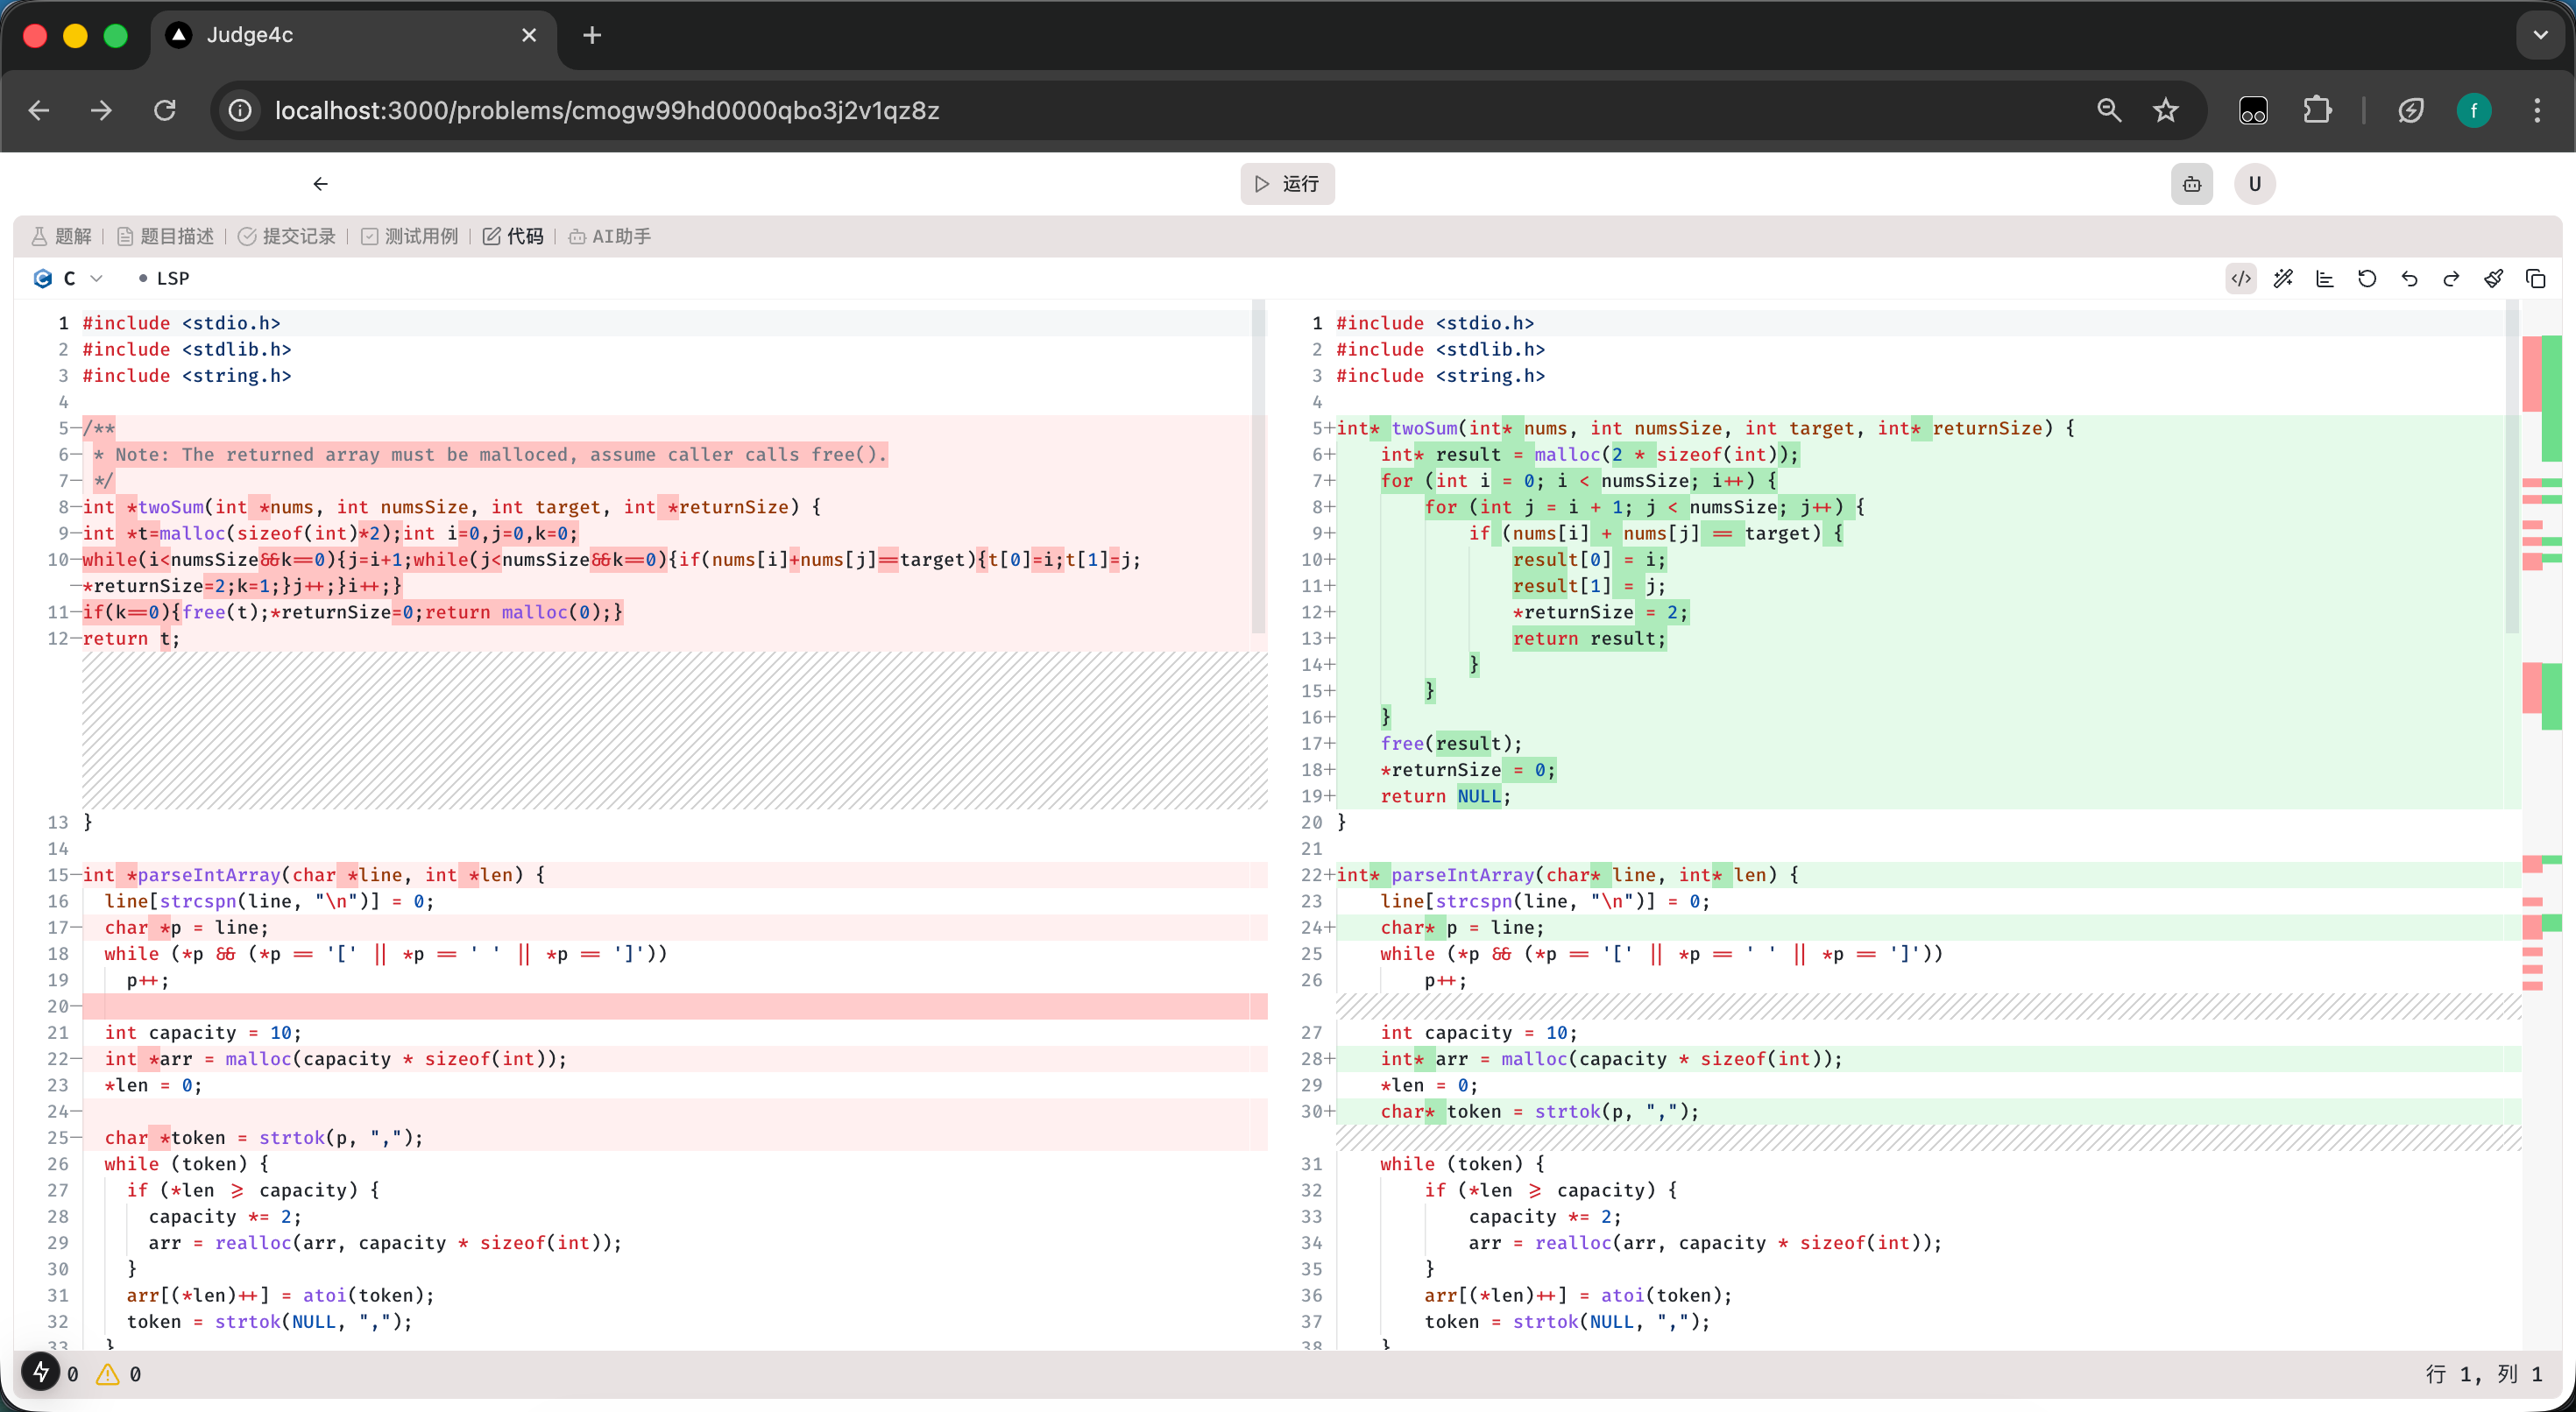
\includegraphics[width=0.96\textwidth]{images/fig6-7.png}
  \caption{优化代码后的 Diff 对比视图截图}
  \label{fig:diff-view}
\end{figure}

\begin{figure}[htbp]
  \centering
  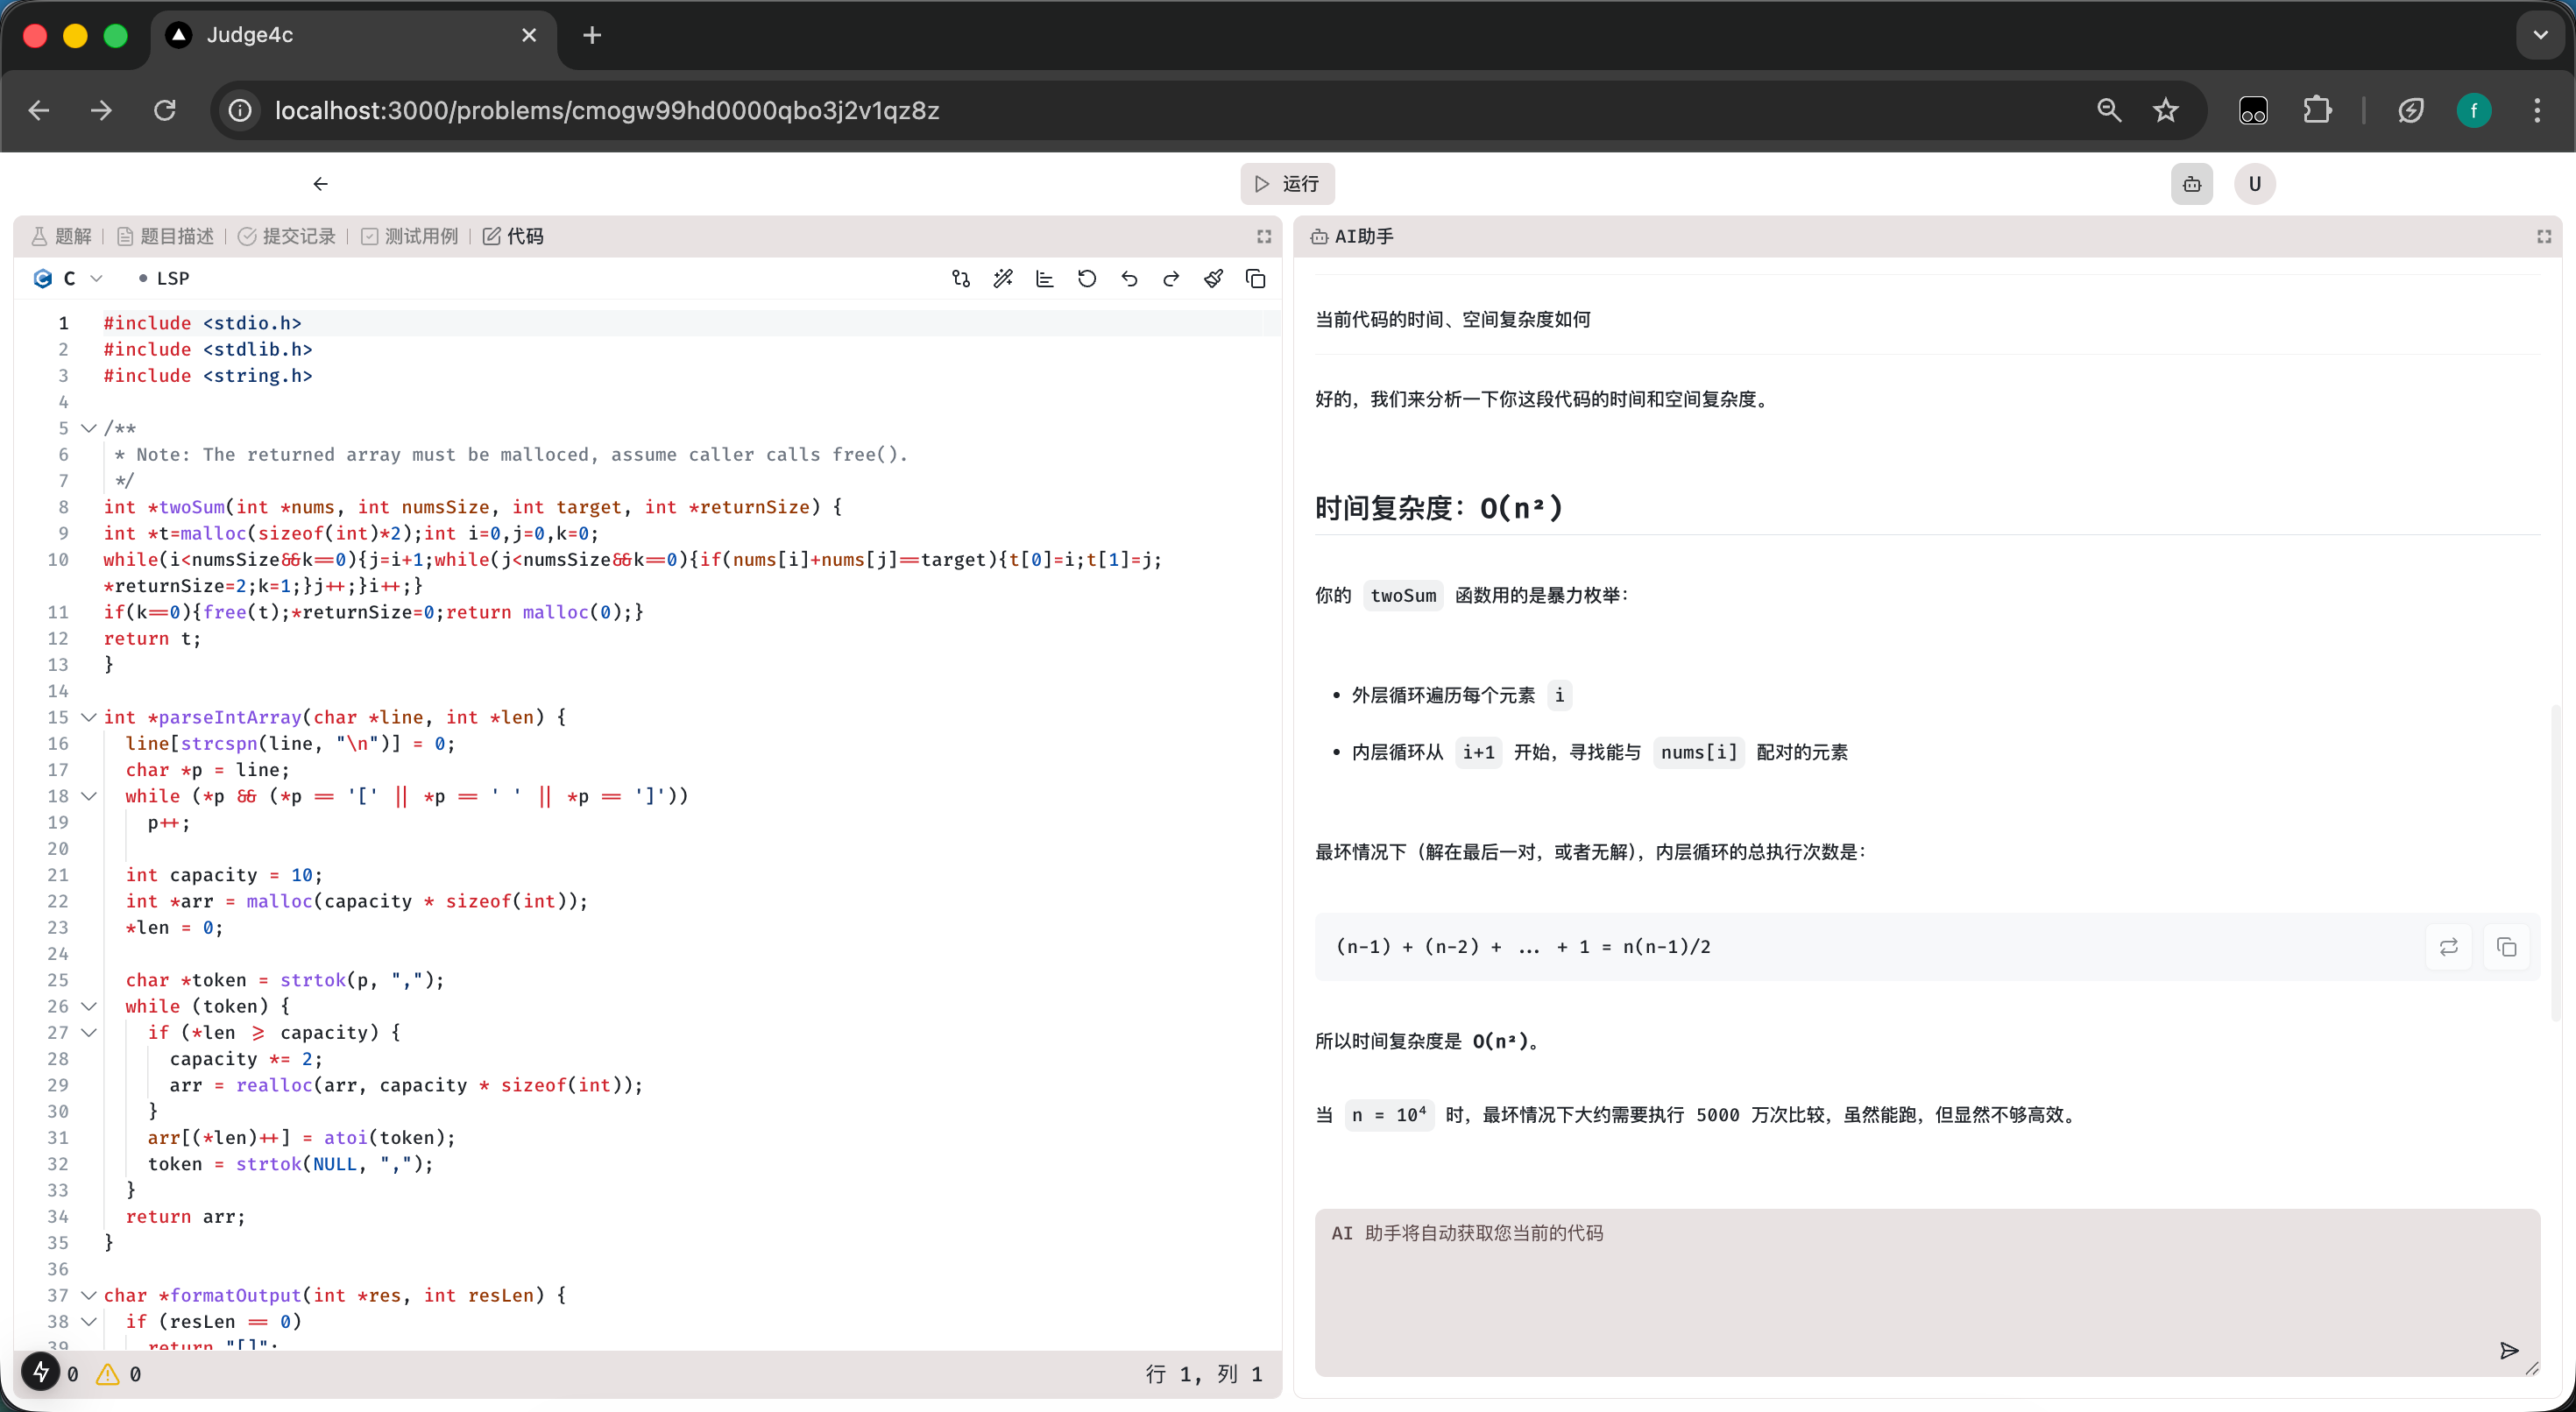
\includegraphics[width=0.96\textwidth]{images/fig6-8.png}
  \caption{AI 助手面板问答截图}
  \label{fig:ai-chat-panel}
\end{figure}

\FloatBarrier
\section{本章小结}

本章给出了测试环境、核心功能、判题正确性、AI 反馈及界面交互的结果。结合正文截图和附录样例代码可见，该系统已经具备可演示、可复核的运行基础，系统核心流程已经跑通，基础判题状态识别基本准确，AI 反馈能够作为补充解释使用。
